
\section{Configuración Experimental} \label{sec:results:setup}

Para evaluar la efectividad de NSGA-II y MOEA/D en la estimación del parámetro de regularización \( \lambda \), se llevaron a cabo experimentos utilizando datos sintéticos generados con base en el modelo de espacio de estados lineales descrito en la Sección \ref{sec:lit:two}. Se analizaron diferentes niveles de varianza del ruido (\( \sigma^2 = 0.0, 10^{-4}, 10^{-3}, 10^{-2}, 10^{-1}, 1.0 \)) para simular condiciones realistas de medición.

El procedimiento experimental incluyó los siguientes pasos:
\begin{enumerate}
    \item Resolución del problema de reconstrucción utilizando el método de la curva L para determinar \( \lambda \).
    \item Exploración de frentes de Pareto de soluciones multiobjetivo utilizando:
    \begin{itemize}
        \item NSGA-II, un algoritmo evolutivo elitista que prioriza la diversidad del frente de Pareto.
        \item MOEA/D, un algoritmo basado en descomposición que equilibra las soluciones a través del frente.
    \end{itemize}
    \item Definición de los siguientes objetivos:
    \begin{enumerate}
        \item Minimización del residual: \( \| \mathbf{y} - \mathbf{H} \mathbf{d} \|_2^2 \),
        \item Minimización de la regularización: \( \| \mathbf{d} \|_2^2 \),
        \item Penalización de valores negativos en \( \mathbf{d} \), para garantizar soluciones físicamente consistentes.
    \end{enumerate}
    \item Reconstrucción del perfil de absorción \( \mathbf{\mu} \) utilizando los valores de \( \lambda \) generados por ambos algoritmos.
    \item Comparación gráfica y cuantitativa de los resultados obtenidos con NSGA-II, MOEA/D y el método de la curva L.
\end{enumerate}

\section{Resultados del Frente de Pareto} \label{sec:results:pareto}

Los frentes de Pareto generados por NSGA-II y MOEA/D proporcionan un conjunto de soluciones que representan distintos compromisos entre los objetivos definidos. Las Figuras \ref{fig:pareto_front_nsga2} y \ref{fig:pareto_front_moead} muestran los frentes de Pareto obtenidos para \( \sigma^2 = 10^{-1} \) utilizando NSGA-II y MOEA/D, respectivamente.

\begin{figure}[H]
    \centering
    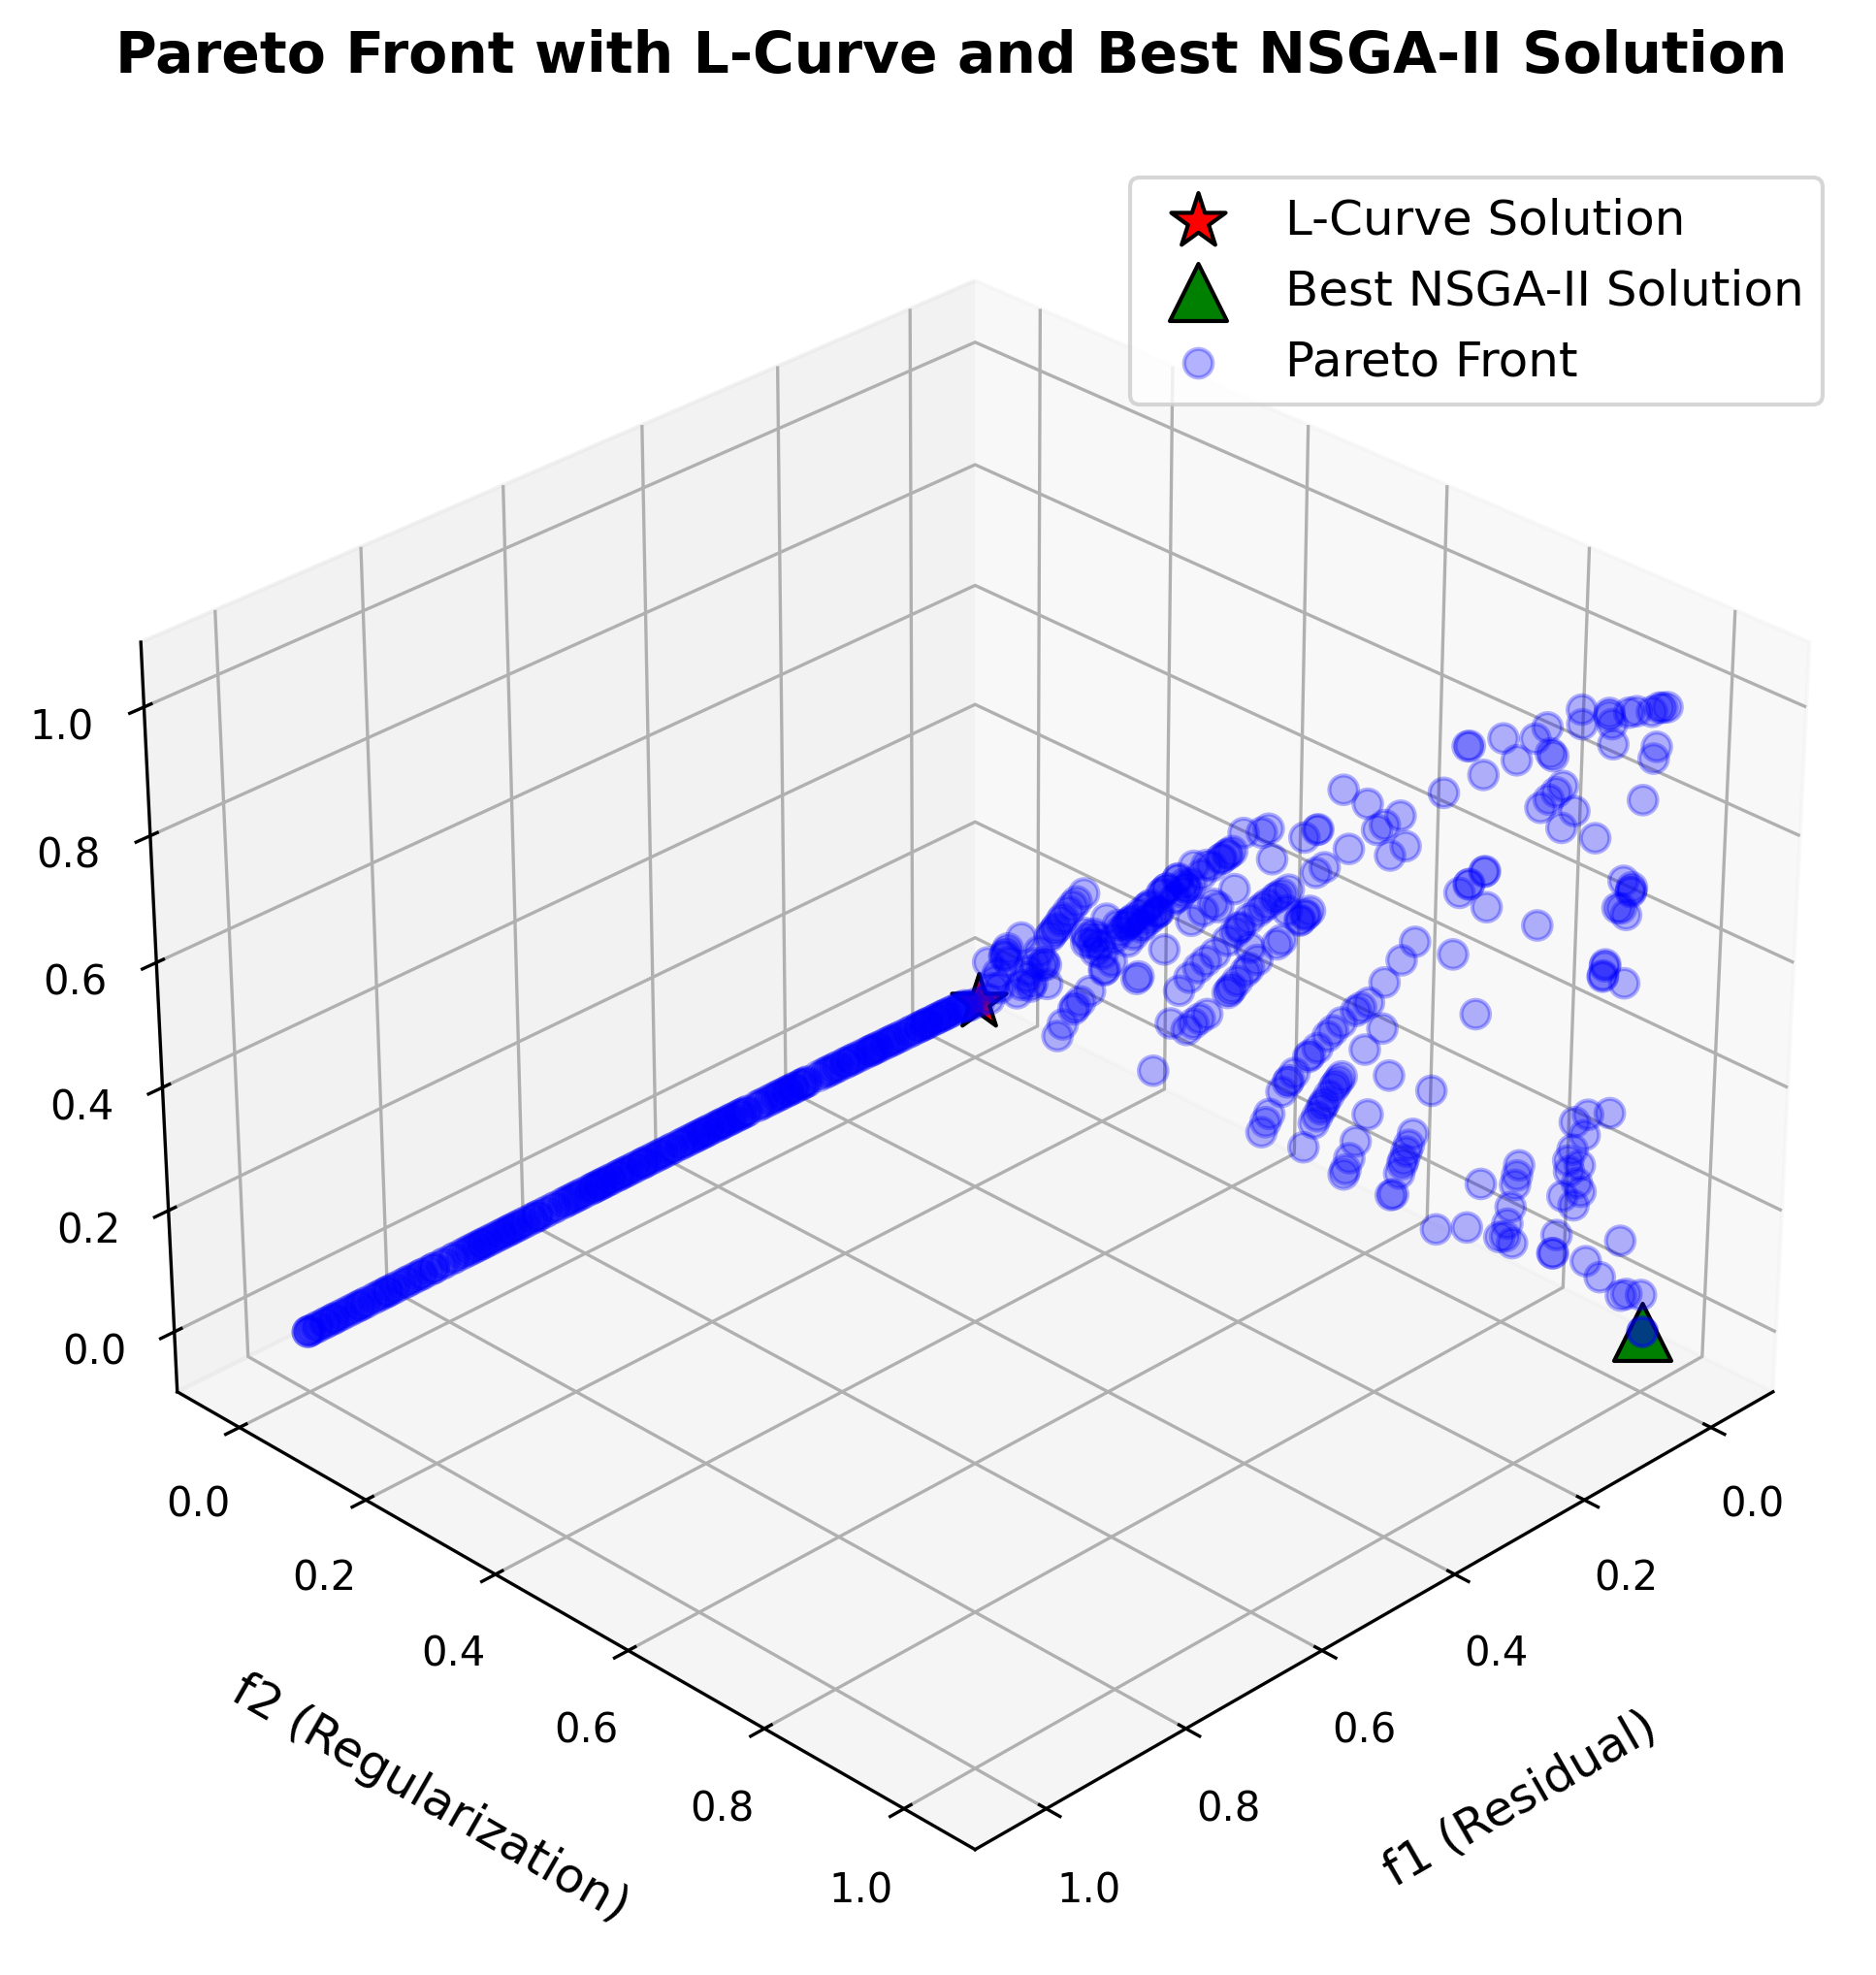
\includegraphics[width=0.8\textwidth]{Images/pareto_front_nsga2.png}
    \caption{Frente de Pareto generado por NSGA-II para \( \lambda \). Cada punto representa un compromiso entre los objetivos.}
    \label{fig:pareto_front_nsga2}
\end{figure}

\begin{figure}[H]
    \centering
    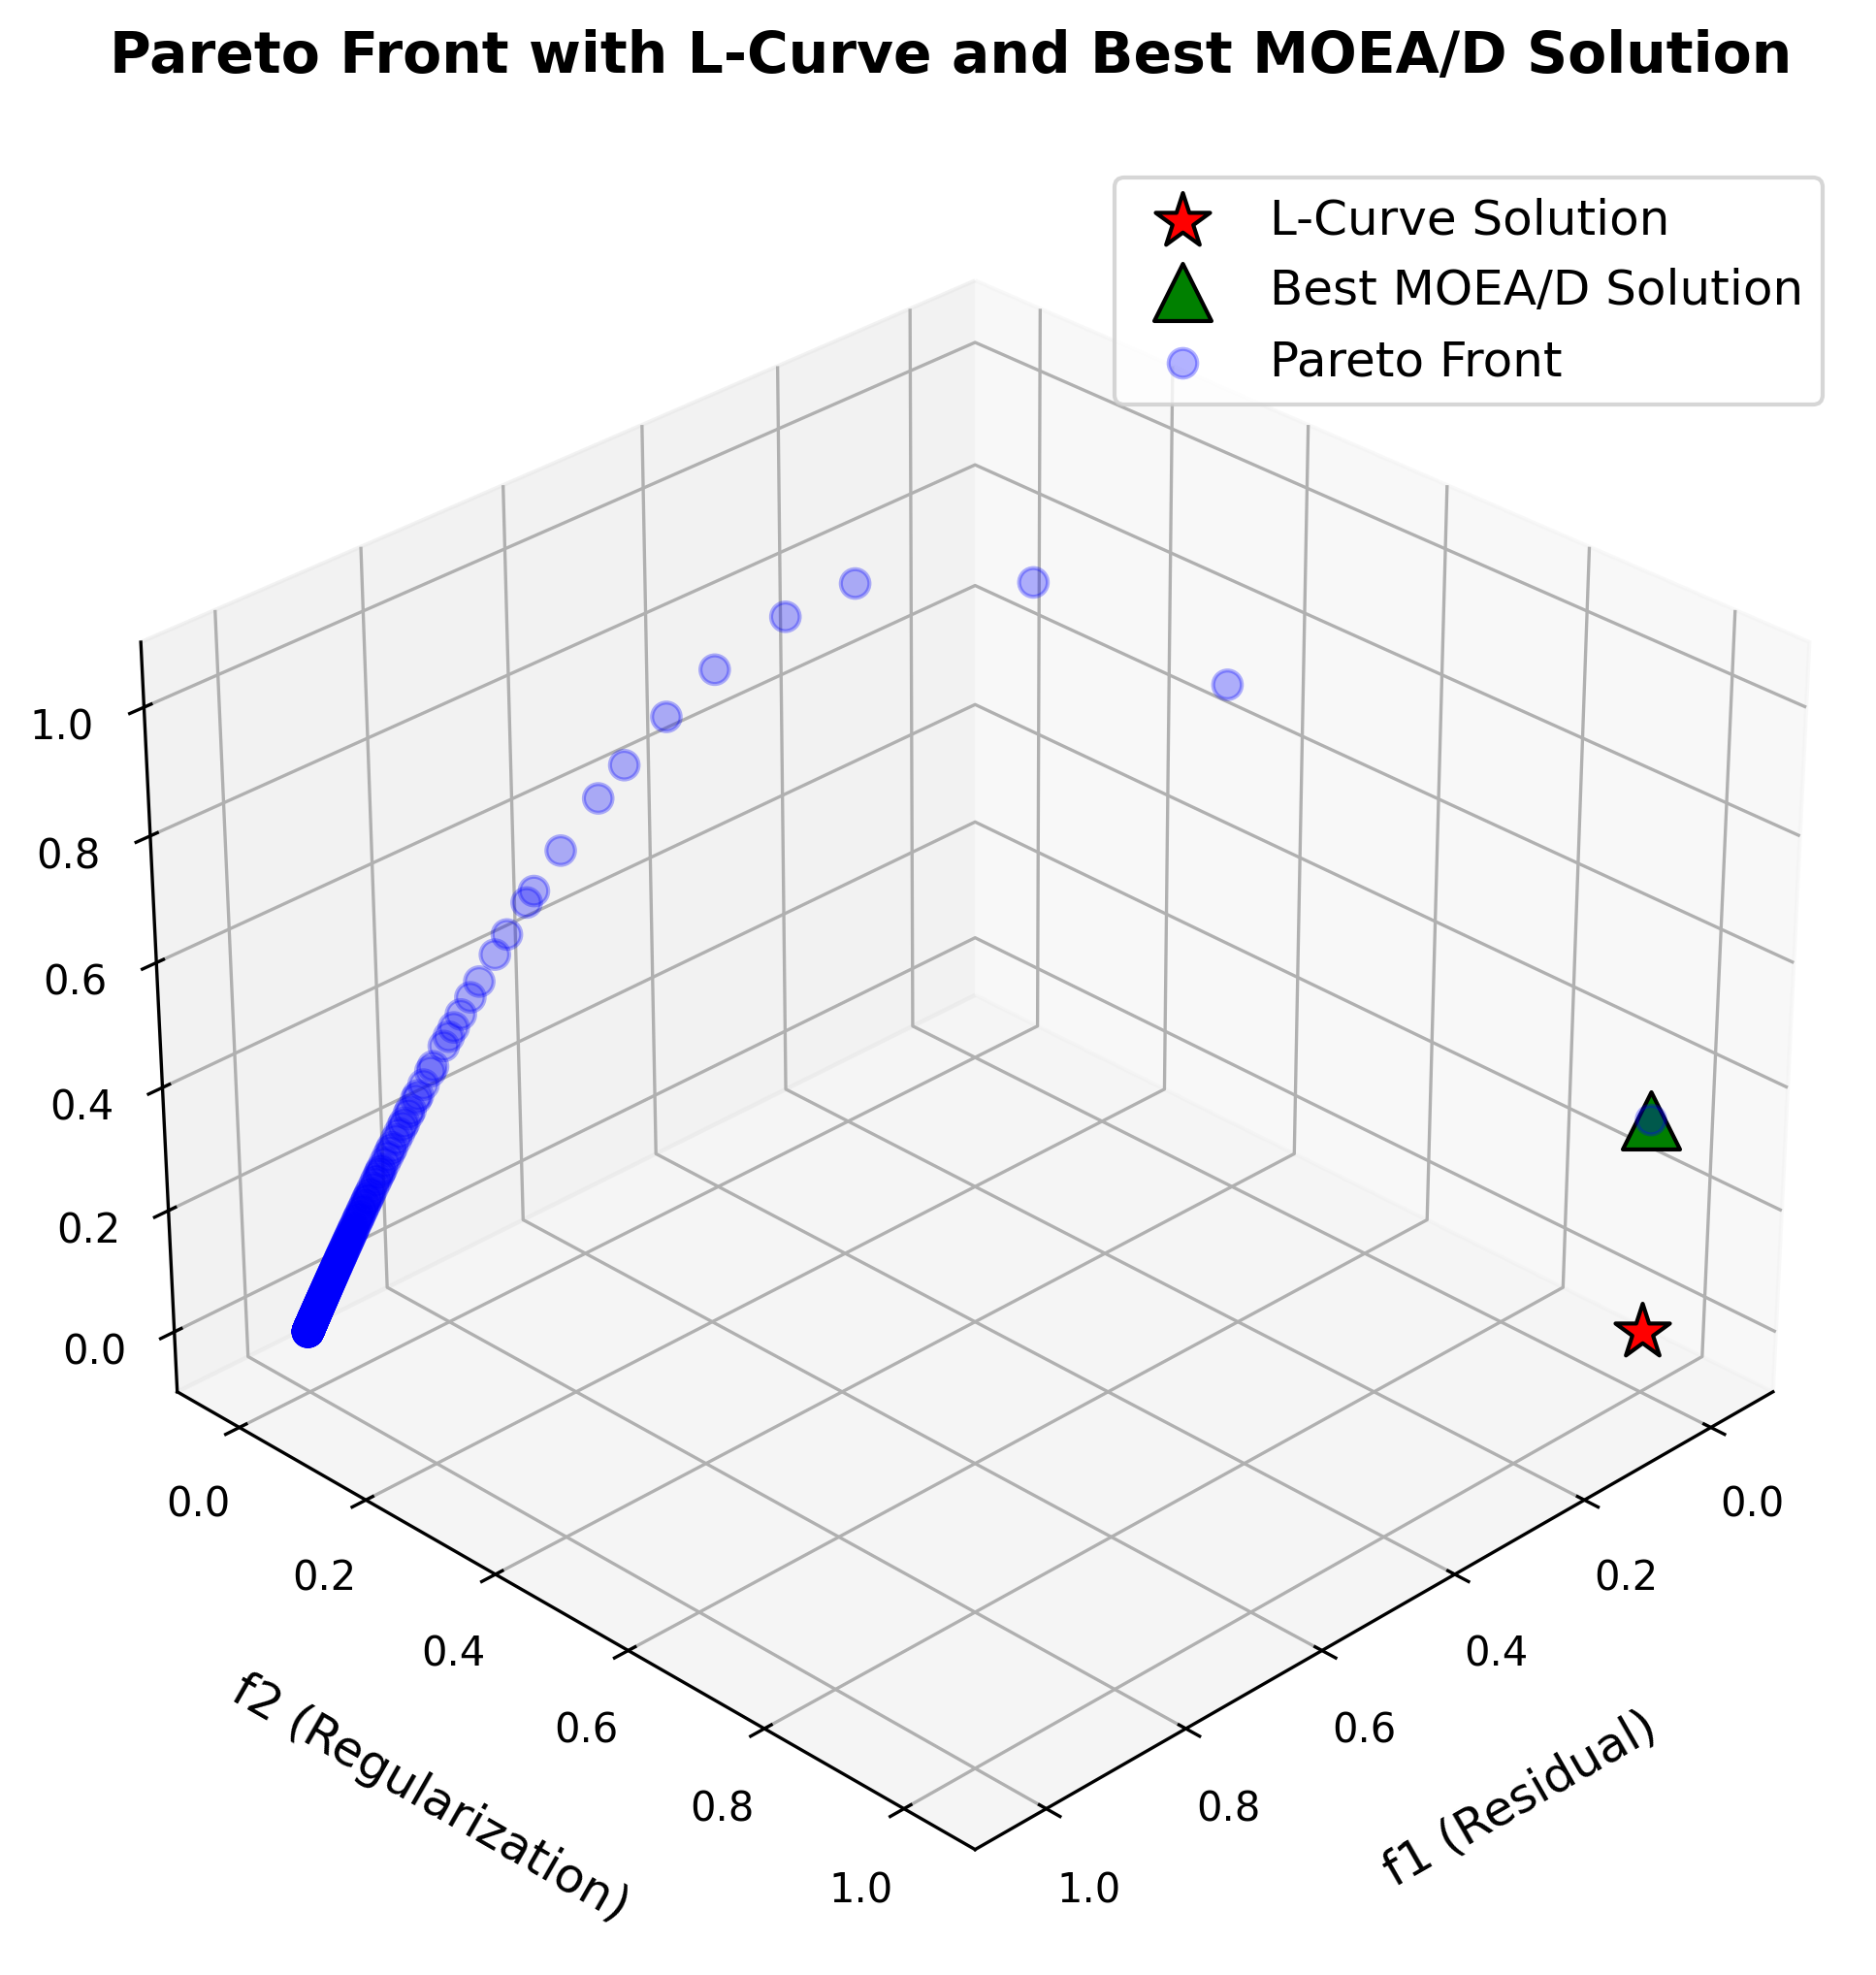
\includegraphics[width=0.8\textwidth]{Images/pareto_front_moead.png}
    \caption{Frente de Pareto generado por MOEA/D para \( \lambda \). Cada punto representa un compromiso entre los objetivos.}
    \label{fig:pareto_front_moead}
\end{figure}

Aunque ambos algoritmos exploran soluciones diversas, MOEA/D genera frentes más equilibrados debido a su enfoque basado en descomposición, mientras que NSGA-II se enfoca más en la diversidad.

\section{Análisis de Clustering de los Frentes de Pareto} \label{sec:results:clustering}

Se realizó un análisis de clustering para interpretar mejor los frentes de Pareto, identificando regiones que representan diferentes compromisos entre los objetivos. Las Figuras \ref{fig:pareto_clustering_nsga2} y \ref{fig:pareto_clustering_moead} muestran los frentes de Pareto agrupados en tres clusters para NSGA-II y MOEA/D, respectivamente.

\begin{figure}[H]
    \centering
    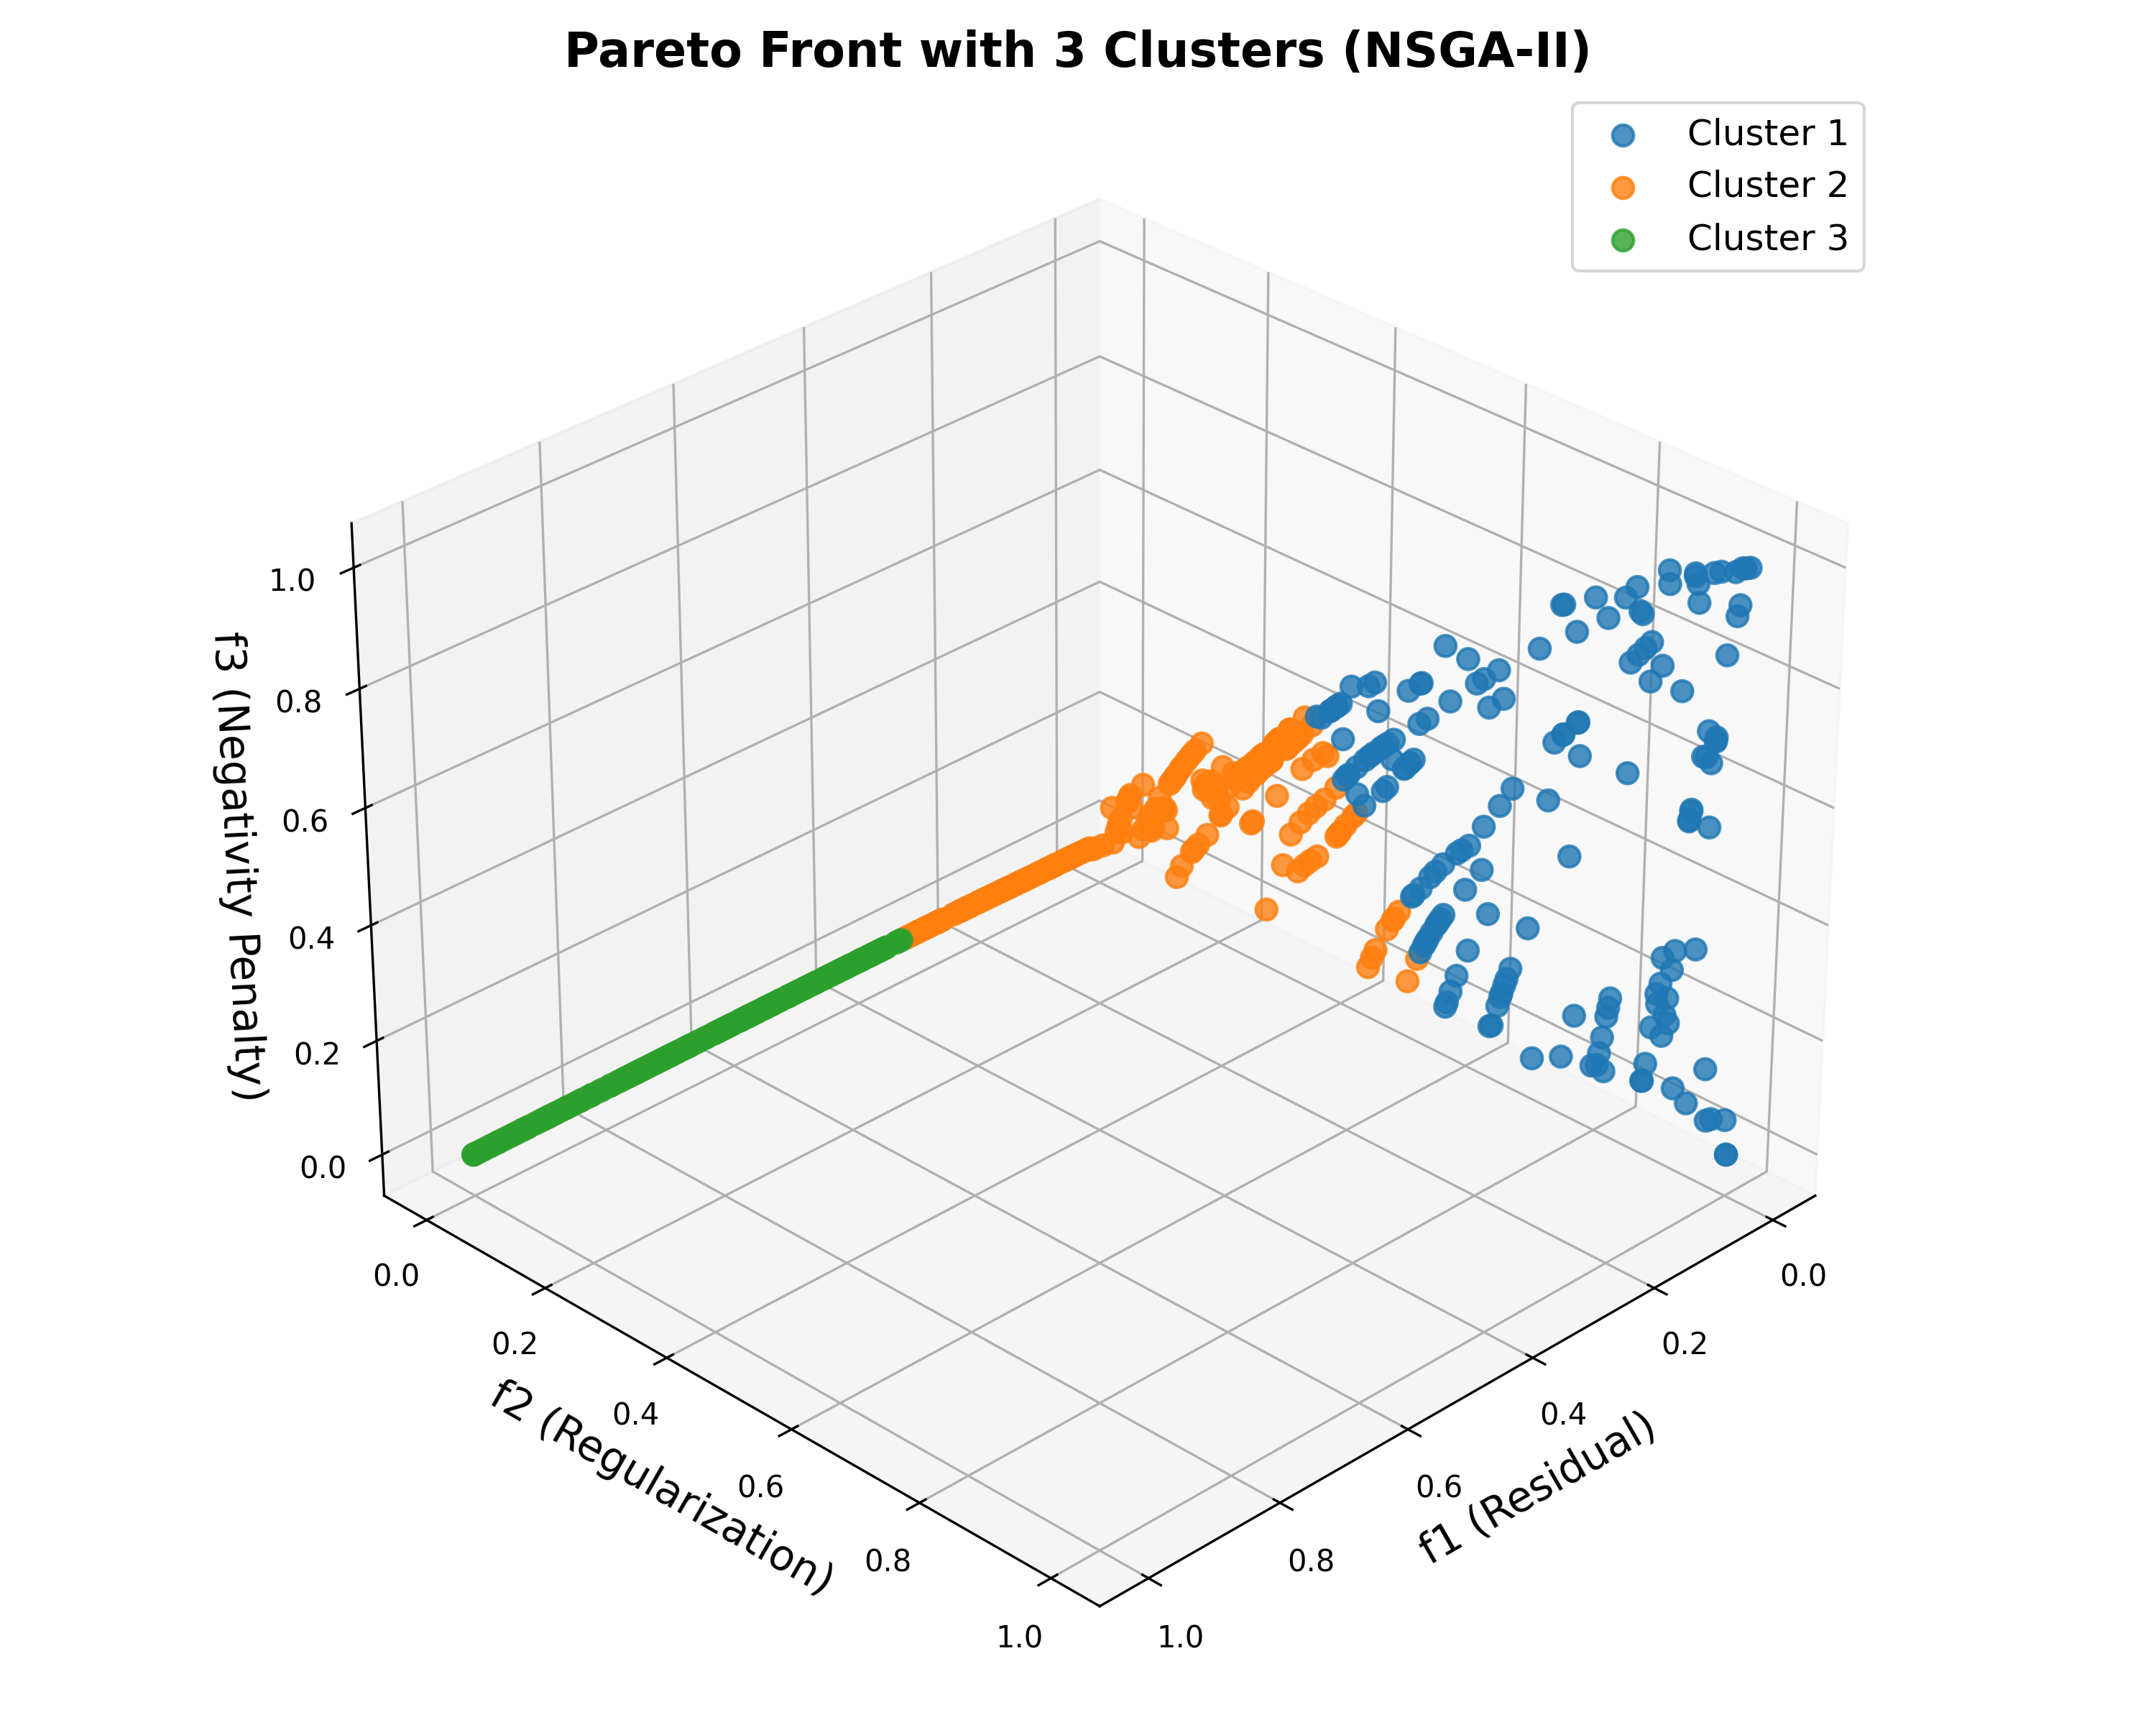
\includegraphics[width=0.8\textwidth]{Images/pareto_clustering_nsga2.png}
    \caption{Clustering del frente de Pareto generado por NSGA-II. Cada color representa un grupo de soluciones con características similares.}
    \label{fig:pareto_clustering_nsga2}
\end{figure}

\begin{figure}[H]
    \centering
    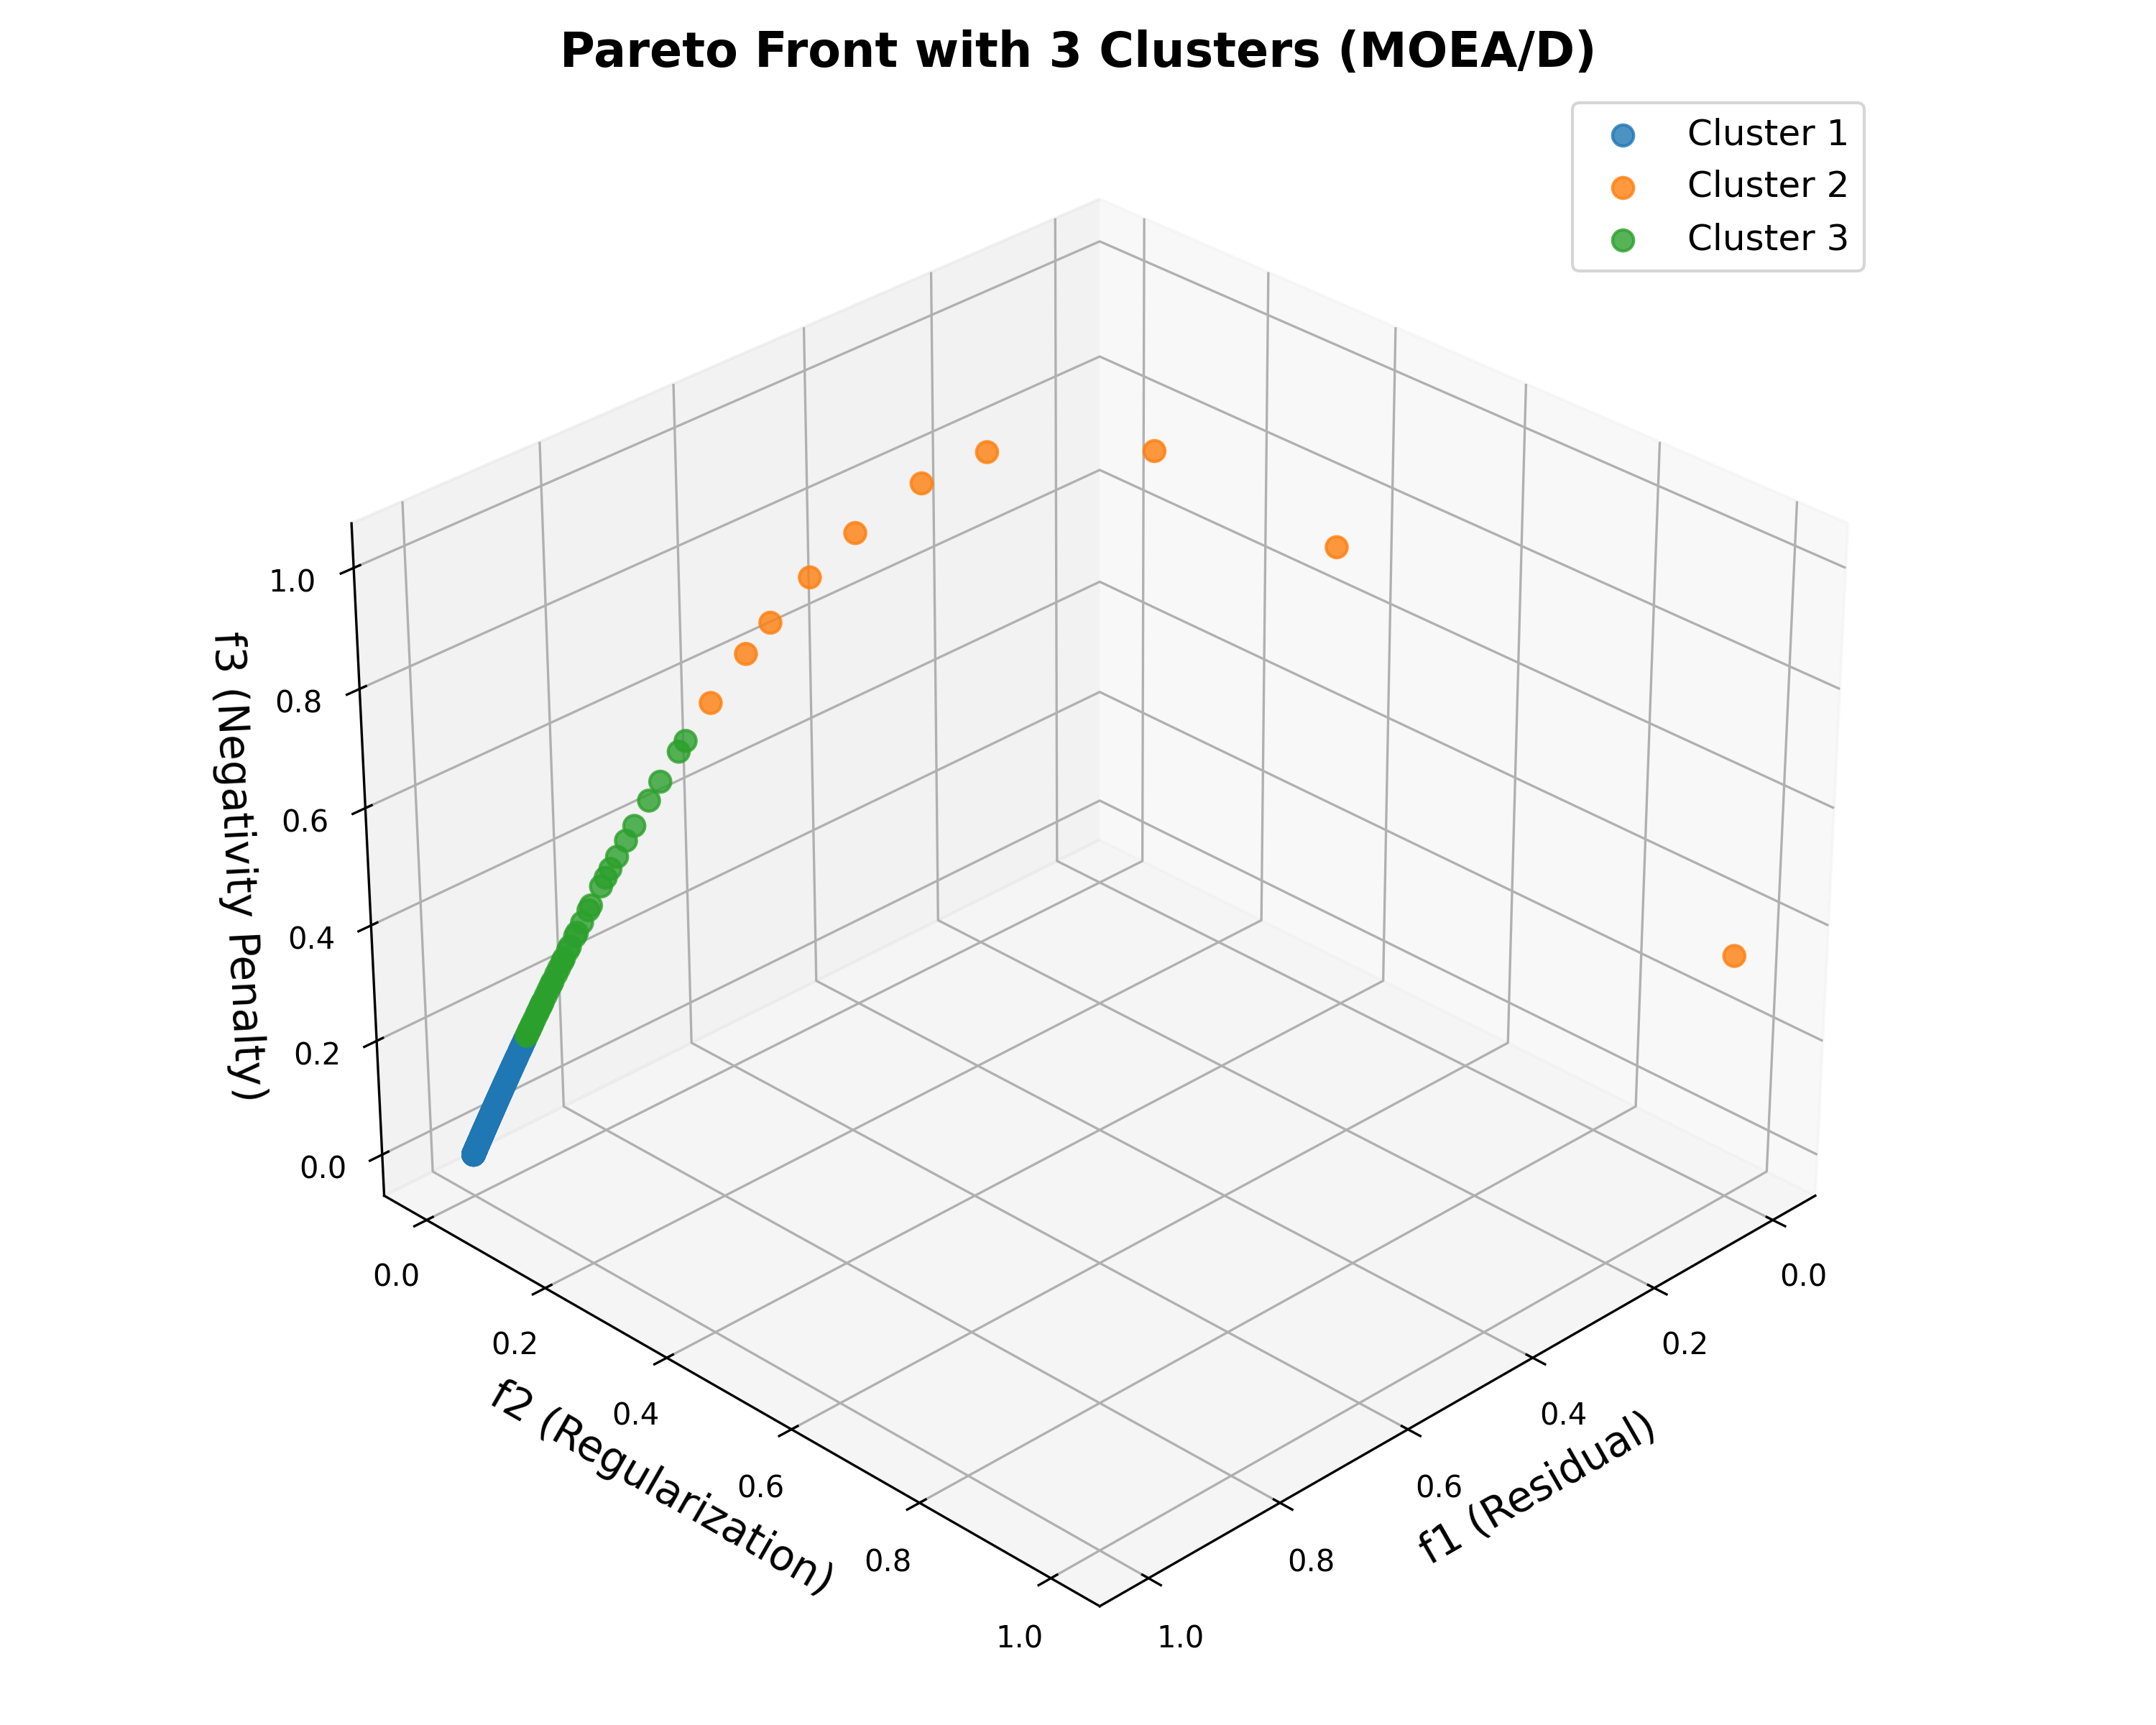
\includegraphics[width=0.8\textwidth]{Images/pareto_clustering_moead.png}
    \caption{Clustering del frente de Pareto generado por MOEA/D. Cada color representa un grupo de soluciones con características similares.}
    \label{fig:pareto_clustering_moead}
\end{figure}

El análisis revela:
\begin{itemize}
    \item NSGA-II ofrece mayor diversidad en regiones dominadas por el residual (\( f_1 \)).
    \item MOEA/D genera soluciones más uniformes en zonas con alta penalización de negatividad (\( f_3 \)).
\end{itemize}

\section{Reconstrucción del Perfil de Absorción} \label{sec:results:reconstruction}

Las Figuras \ref{fig:reconstruction_profiles_nsga2} y \ref{fig:reconstruction_profiles_moead} presentan los perfiles de absorción \( \mathbf{\mu} \) reconstruidos utilizando los valores de \( \lambda \) obtenidos con NSGA-II y MOEA/D para \( \sigma^2 = 10^{-1} \), respectivamente.

\begin{figure}[H]
    \centering
    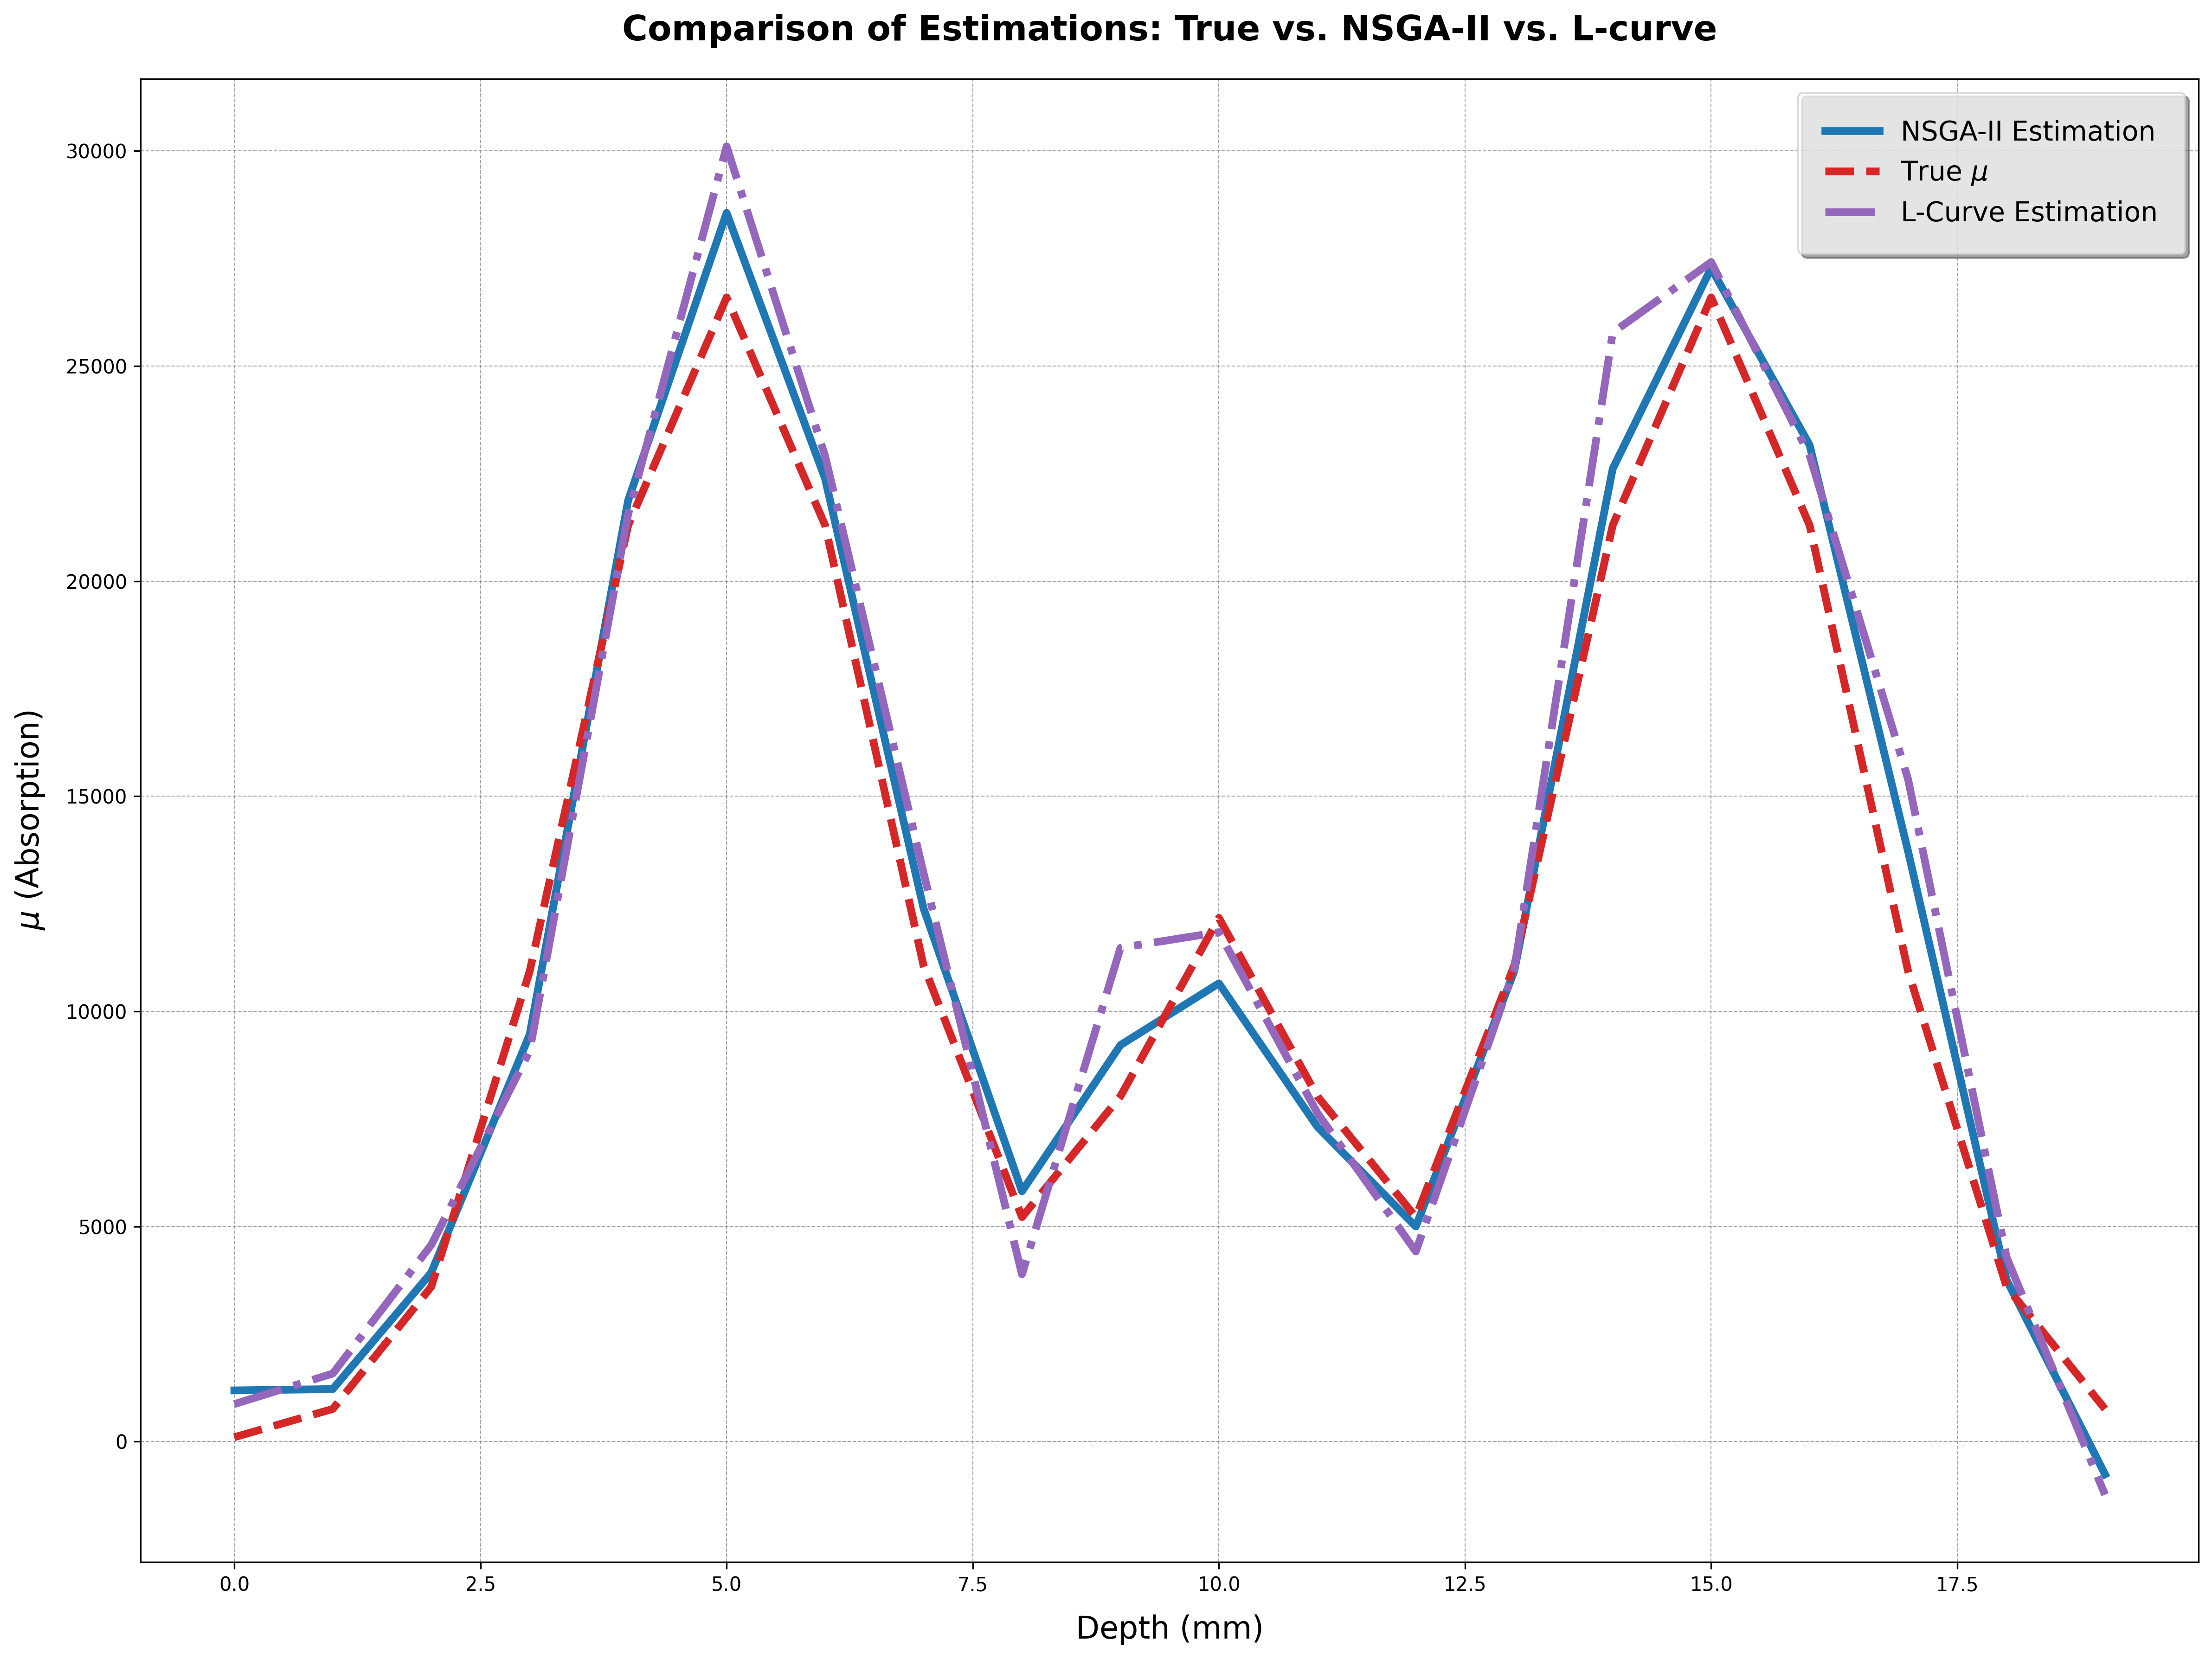
\includegraphics[width=0.8\textwidth]{Images/reconstruction_profiles_nsga2.png}
    \caption{Perfiles de absorción reconstruidos utilizando NSGA-II. La curva azul representa el perfil real y la curva roja corresponde a la solución reconstruida.}
    \label{fig:reconstruction_profiles_nsga2}
\end{figure}

\begin{figure}[H]
    \centering
    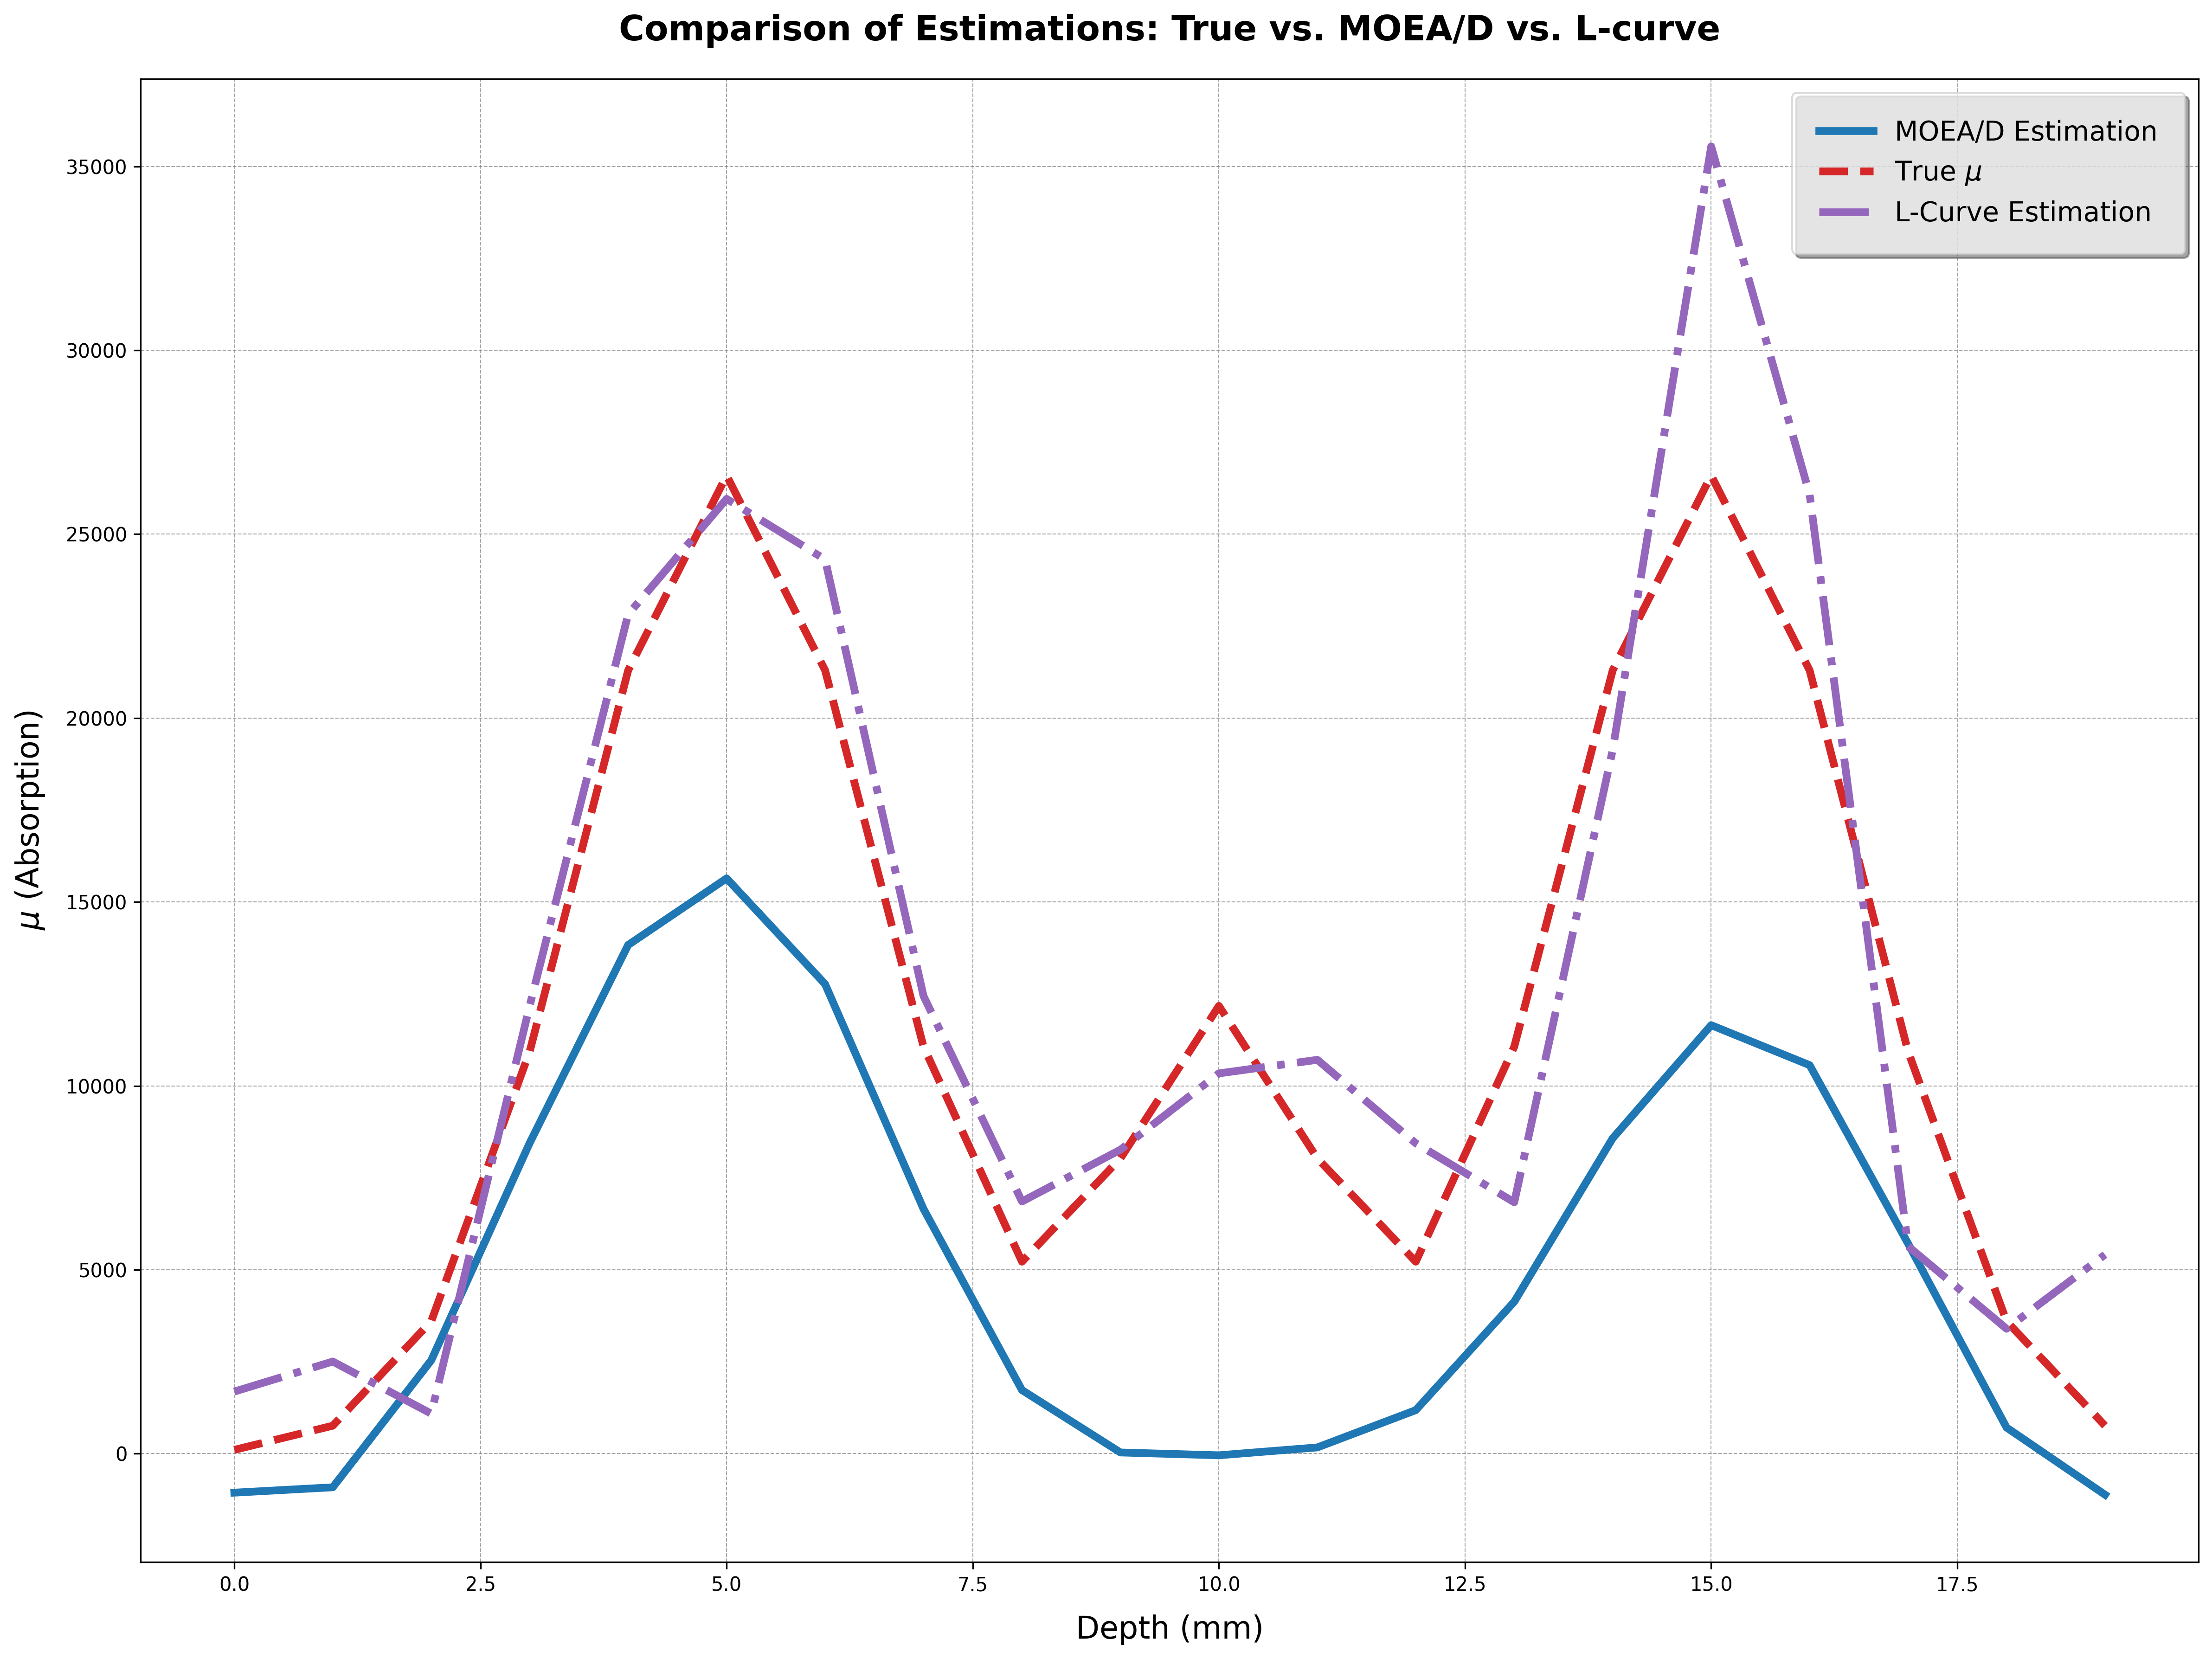
\includegraphics[width=0.8\textwidth]{Images/reconstruction_profiles_moead.png}
    \caption{Perfiles de absorción reconstruidos utilizando MOEA/D. La curva azul representa el perfil real y la curva verde corresponde a la solución reconstruida.}
    \label{fig:reconstruction_profiles_moead}
\end{figure}

Ambos métodos producen reconstrucciones físicamente consistentes en comparación con el método de la curva L, pero MOEA/D genera perfiles más estables en condiciones de ruido elevado.

\section{Resultados del Hipervolumen} \label{sec:results:hypervolume}

El hipervolumen se utilizó como una métrica clave para evaluar la calidad y la diversidad del frente de Pareto generado por NSGA-II y MOEA/D para \( \sigma^2 = 10^{-1} \). Este indicador mide el espacio objetivo dominado por las soluciones en el frente de Pareto en relación con un punto de referencia (\( [10,10,10] \)). Por lo tanto, un mayor hipervolumen indica una mejor representación y diversidad del frente.

\begin{figure}[H]
    \centering
    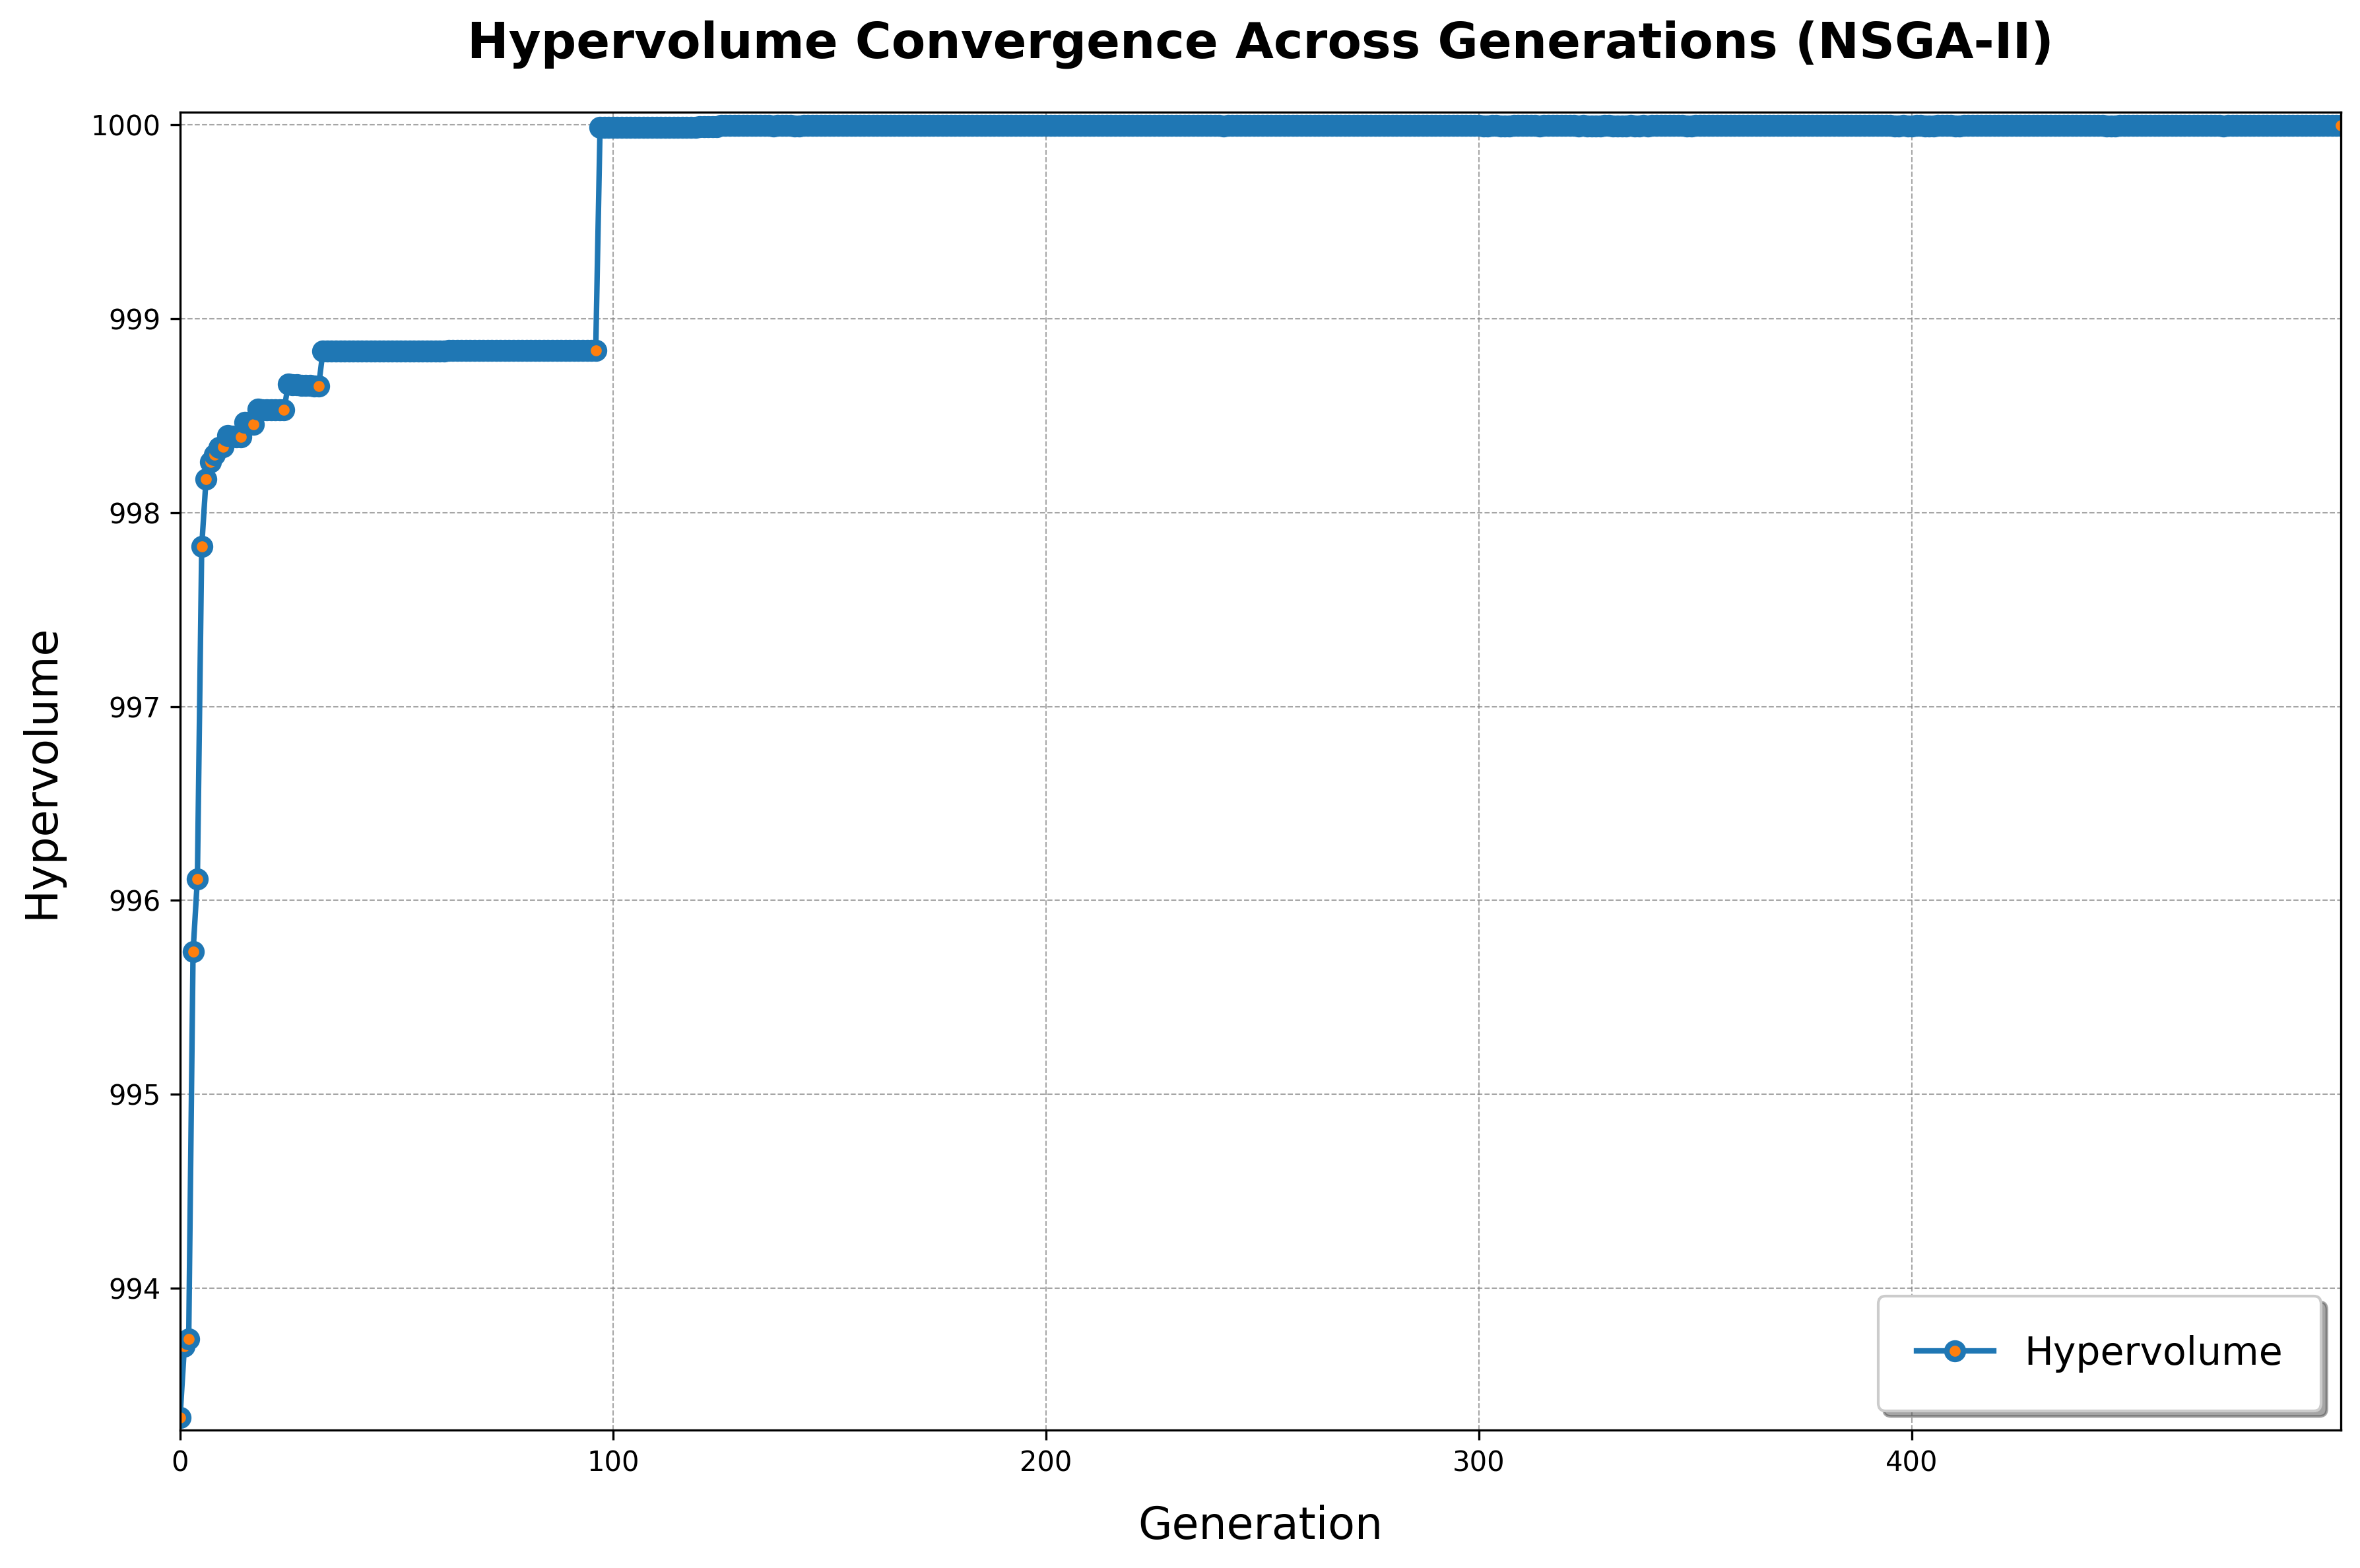
\includegraphics[width=0.8\textwidth]{Images/hypervolume_nsga2.png}
    \caption{Convergencia del hipervolumen a lo largo de generaciones para NSGA-II.}
    \label{fig:hypervolume_nsga2}
\end{figure}

\begin{figure}[H]
    \centering
    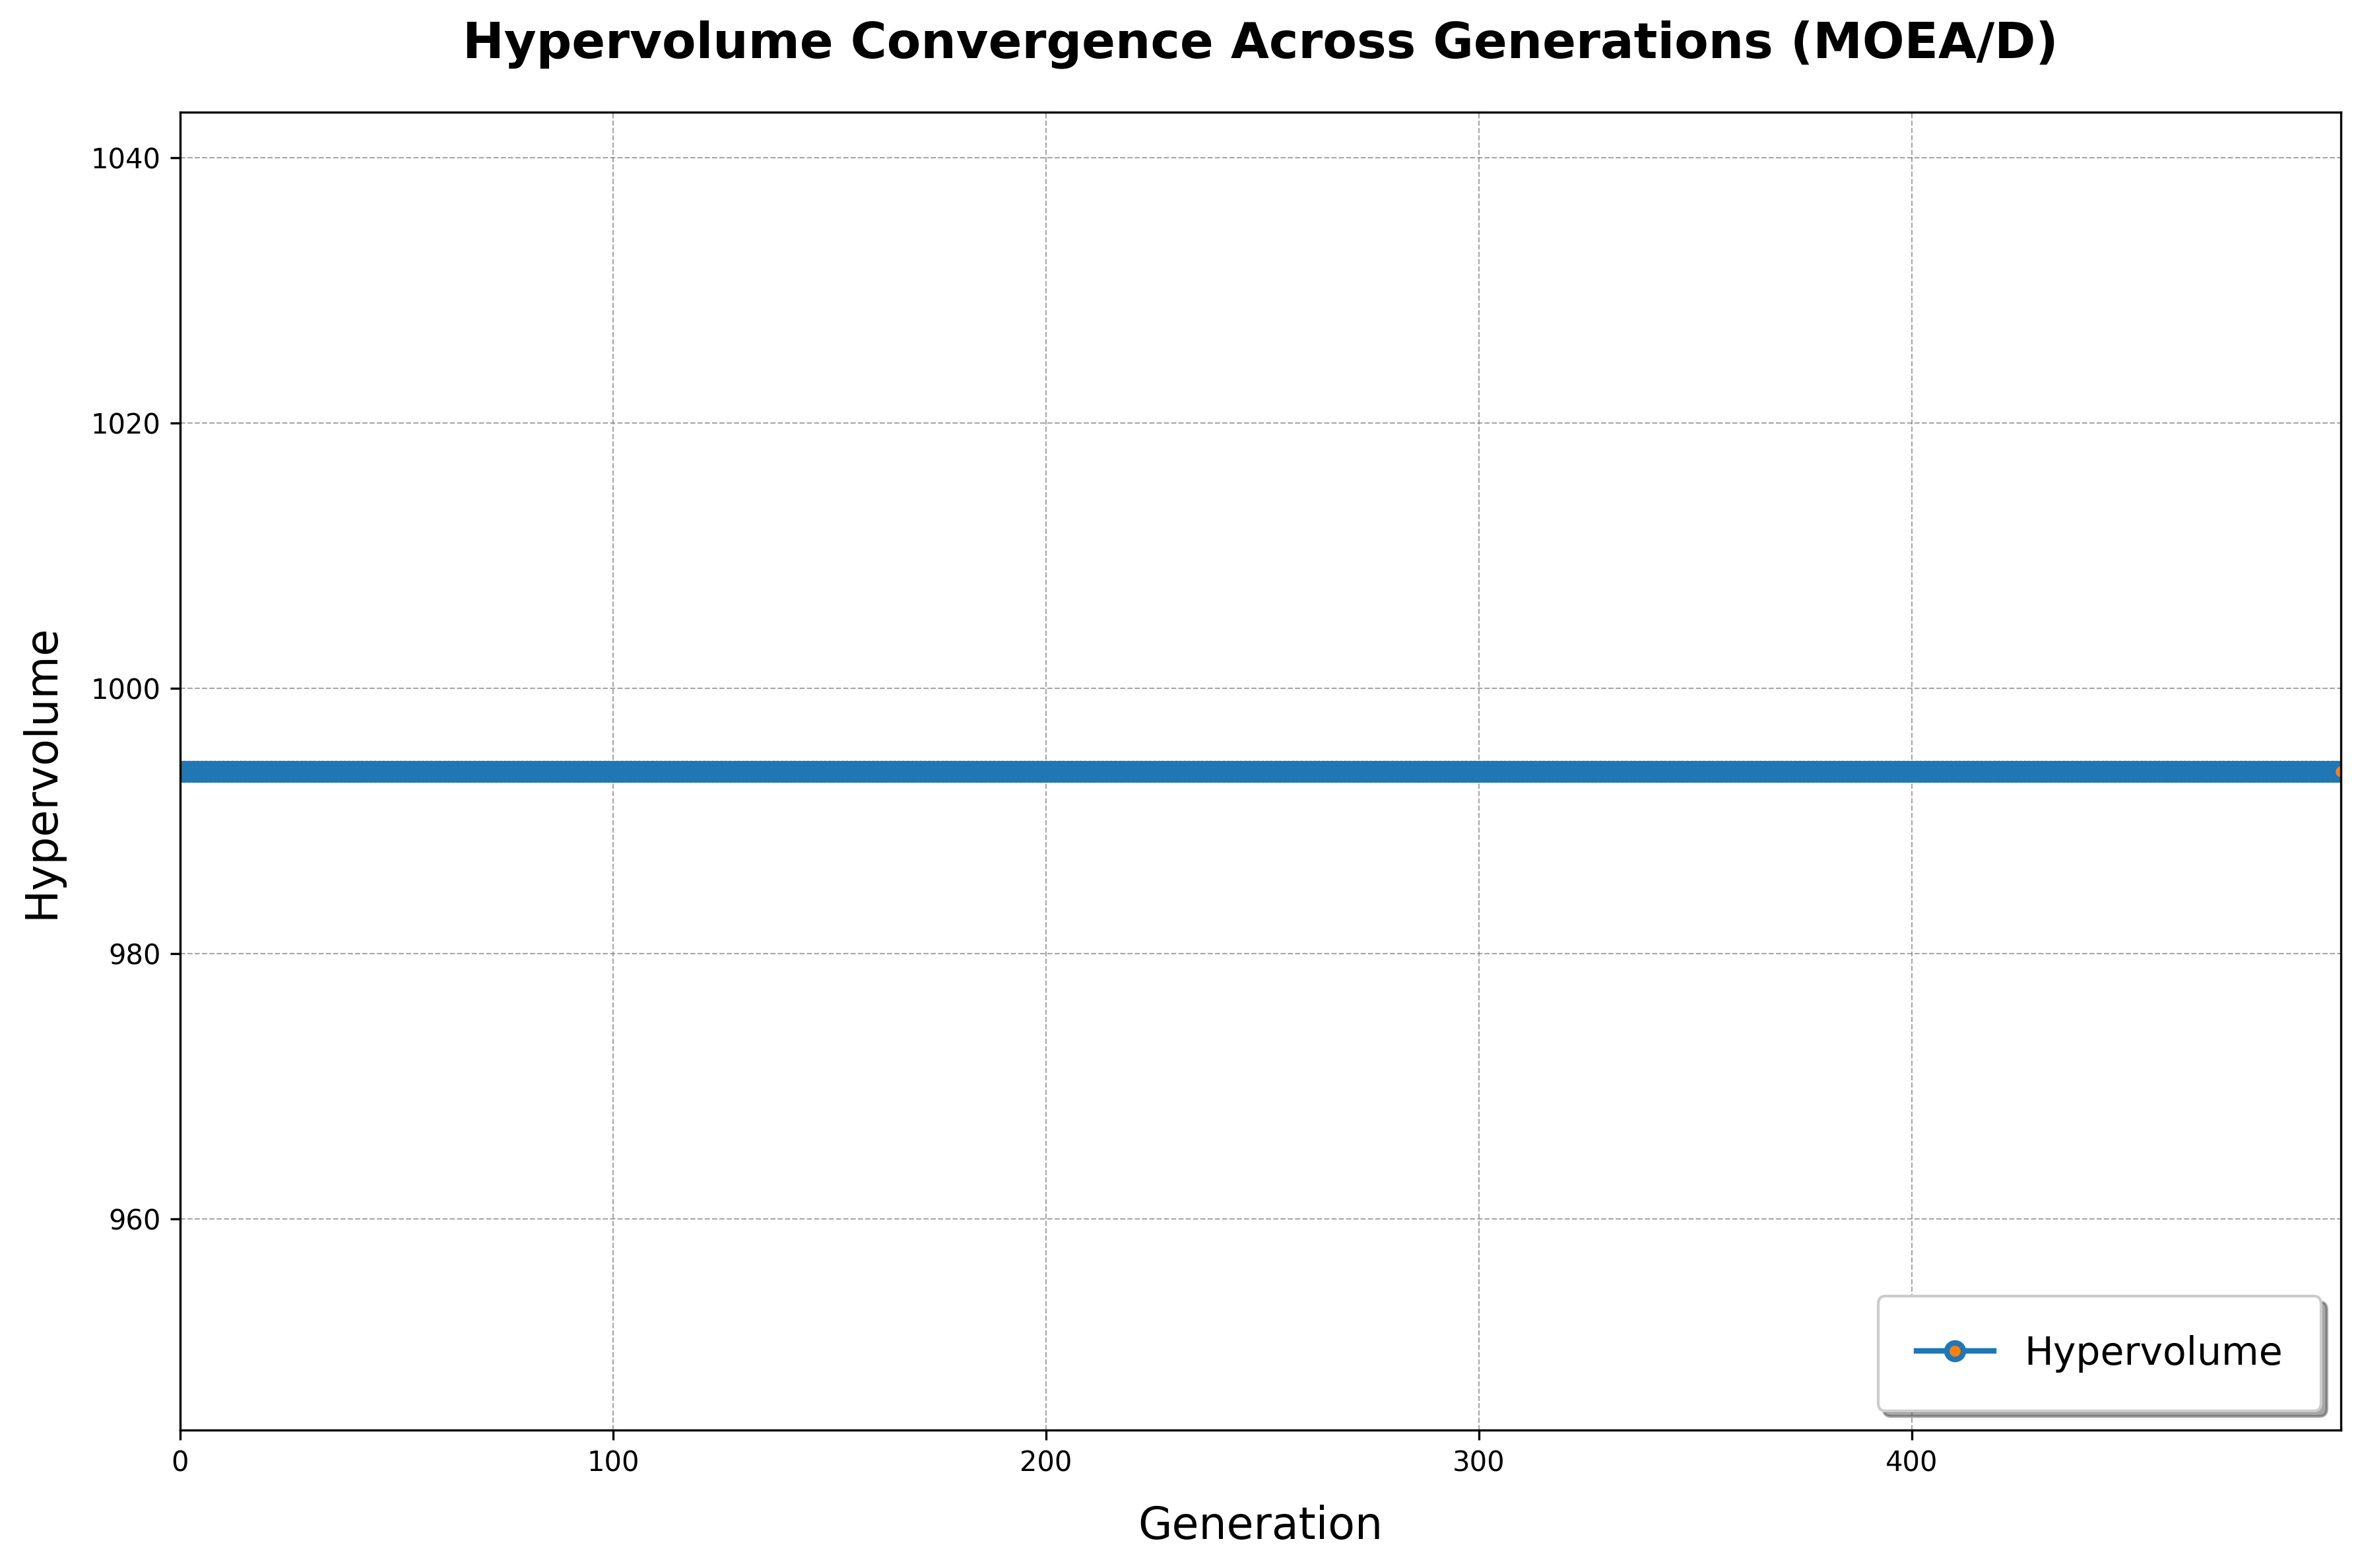
\includegraphics[width=0.8\textwidth]{Images/hypervolume_moead.png}
    \caption{Convergencia del hipervolumen a lo largo de generaciones para MOEA/D.}
    \label{fig:hypervolume_moead}
\end{figure}

\textbf{Observaciones}

\textbf{NSGA-II:} La Figura \ref{fig:hypervolume_nsga2} muestra que el hipervolumen generado por NSGA-II converge rápidamente a un valor máximo alrededor de las primeras 50 generaciones. Esto indica que NSGA-II es capaz de explorar eficientemente el espacio objetivo y alcanzar un frente de Pareto de alta calidad en pocas iteraciones. Además, la variación inicial del hipervolumen refleja la diversidad de soluciones generadas durante las primeras generaciones, lo que sugiere un enfoque efectivo para equilibrar los objetivos definidos.

\textbf{MOEA/D:} Por otro lado, la Figura \ref{fig:hypervolume_moead} presenta un comportamiento notablemente constante del hipervolumen a lo largo de todas las generaciones. Aunque este patrón podría interpretarse inicialmente como una falta de progreso, el análisis de las soluciones generadas revela que MOEA/D produce frentes de Pareto altamente uniformes y equilibrados desde el inicio de la ejecución. Este comportamiento destaca la eficiencia de MOEA/D para mantener una representación estable del espacio objetivo, aunque su dinámica de convergencia requiere un análisis más detallado para comprender completamente sus implicaciones.

\textbf{Consideraciones Finales:}

El comportamiento del hipervolumen en MOEA/D, aunque constante, no debe ser interpretado como una deficiencia en su desempeño. Por el contrario, las soluciones generadas por MOEA/D muestran una alta calidad y diversidad, lo que sugiere que el algoritmo logra rápidamente un equilibrio óptimo en el frente de Pareto. Este comportamiento podría deberse a la naturaleza de su enfoque basado en descomposición, que prioriza soluciones distribuidas de manera uniforme en el espacio objetivo desde el inicio.

En contraste, NSGA-II presenta una convergencia más dinámica, lo que refleja su capacidad para explorar y refinar continuamente el frente de Pareto. Ambos algoritmos ofrecen ventajas complementarias, y su uso debe ser considerado en función de las necesidades específicas del problema, como la rapidez en la convergencia o la uniformidad de las soluciones.


\section{Comparación entre NSGA-II, MOEA/D y la Curva L} \label{sec:results:comparison}

En esta sección se evalúan las soluciones obtenidas mediante NSGA-II, MOEA/D y la solución propuesta por la curva L. La Tabla \ref{tab:comparison_algorithms} resume los valores de los objetivos normalizados para cada metodología para \( \sigma^2 = 10^{-1} \).

\begin{table}[h]
    \centering
    \begin{tabular}{lccc}
        \toprule
        \textbf{Método} & \textbf{Fidelidad (\( f_1 \))} & \textbf{Regularización (\( f_2 \))} & \textbf{Negatividad (\( f_3 \))} \\
        \midrule
        NSGA-II (mejor solución) & 0.000 & 1.000 & 0.000 \\
        MOEA/D (mejor solución) & 0.000 & 1.000 & 0.347 \\
        Curva L & 0.00063 & 0.0071 & 0.0001 \\
        \bottomrule
    \end{tabular}
    \caption{Comparación de las métricas entre NSGA-II, MOEA/D y la curva L. Los valores están normalizados para permitir una evaluación directa.}
    \label{tab:comparison_algorithms}
\end{table}

\noindent
\textbf{Observaciones:}
\begin{itemize}
    \item \textbf{NSGA-II:} Este algoritmo generó la solución con los mejores valores de fidelidad (\( f_1 \)) y negatividad (\( f_3 \)), destacándose en situaciones donde la prioridad es maximizar la precisión y garantizar la consistencia física de la solución.
    \item \textbf{MOEA/D:} Aunque alcanzó valores similares en fidelidad (\( f_1 \)) y regularización (\( f_2 \)) en comparación con NSGA-II, este algoritmo ofreció soluciones con un balance más equitativo entre los tres objetivos, lo que puede ser beneficioso en aplicaciones donde la penalización de la negatividad (\( f_3 \)) no sea tan estricta.
    \item \textbf{Curva L:} Este enfoque tradicional produjo soluciones menos competitivas en todos los objetivos, ya que se centra únicamente en encontrar un compromiso entre fidelidad y regularización, sin considerar objetivos adicionales como la penalización de valores negativos. Sin embargo, destaca por su simplicidad y bajo costo computacional.
\end{itemize}

La selección de las "mejores" soluciones se realizó utilizando un sistema de puntuación ponderado, donde se asignó mayor importancia a la fidelidad (\( f_1 \)) y la regularización (\( f_2 \)), mientras que se aplicó una penalización significativa a la negatividad (\( f_3 \)). Las ponderaciones utilizadas fueron \([0.6, 0.1, 0.3]\), reflejando la prioridad otorgada a cada objetivo en el análisis.

% \noindent
% \textbf{Análisis Comparativo:}

% NSGA-II y MOEA/D muestran una ventaja significativa frente a la curva L al permitir una exploración más amplia y detallada de los compromisos entre objetivos. MOEA/D se distingue por su capacidad para equilibrar objetivos, mientras que NSGA-II es ideal para priorizar fidelidad y minimizar negatividad. Por otro lado, la curva L sigue siendo útil como referencia inicial debido a su simplicidad, aunque carece de la flexibilidad y adaptabilidad que ofrecen los algoritmos evolutivos.

% Estos resultados subrayan la importancia de elegir el enfoque de optimización según los requisitos específicos del problema. En aplicaciones donde la calidad física de las soluciones y el manejo de restricciones son prioritarios, NSGA-II y MOEA/D son opciones superiores, mientras que la curva L podría ser más adecuada para configuraciones iniciales o en problemas menos complejos.

\section{Impacto del Ruido en el RMSE} \label{sec:results:noise}

Las Figuras \ref{fig:rmse_nsga2} y \ref{fig:rmse_moead} muestran el RMSE promedio obtenido para diferentes niveles de varianza del ruido (\( \sigma^2 \)) utilizando NSGA-II y MOEA/D, respectivamente.

\begin{figure}[H]
    \centering
    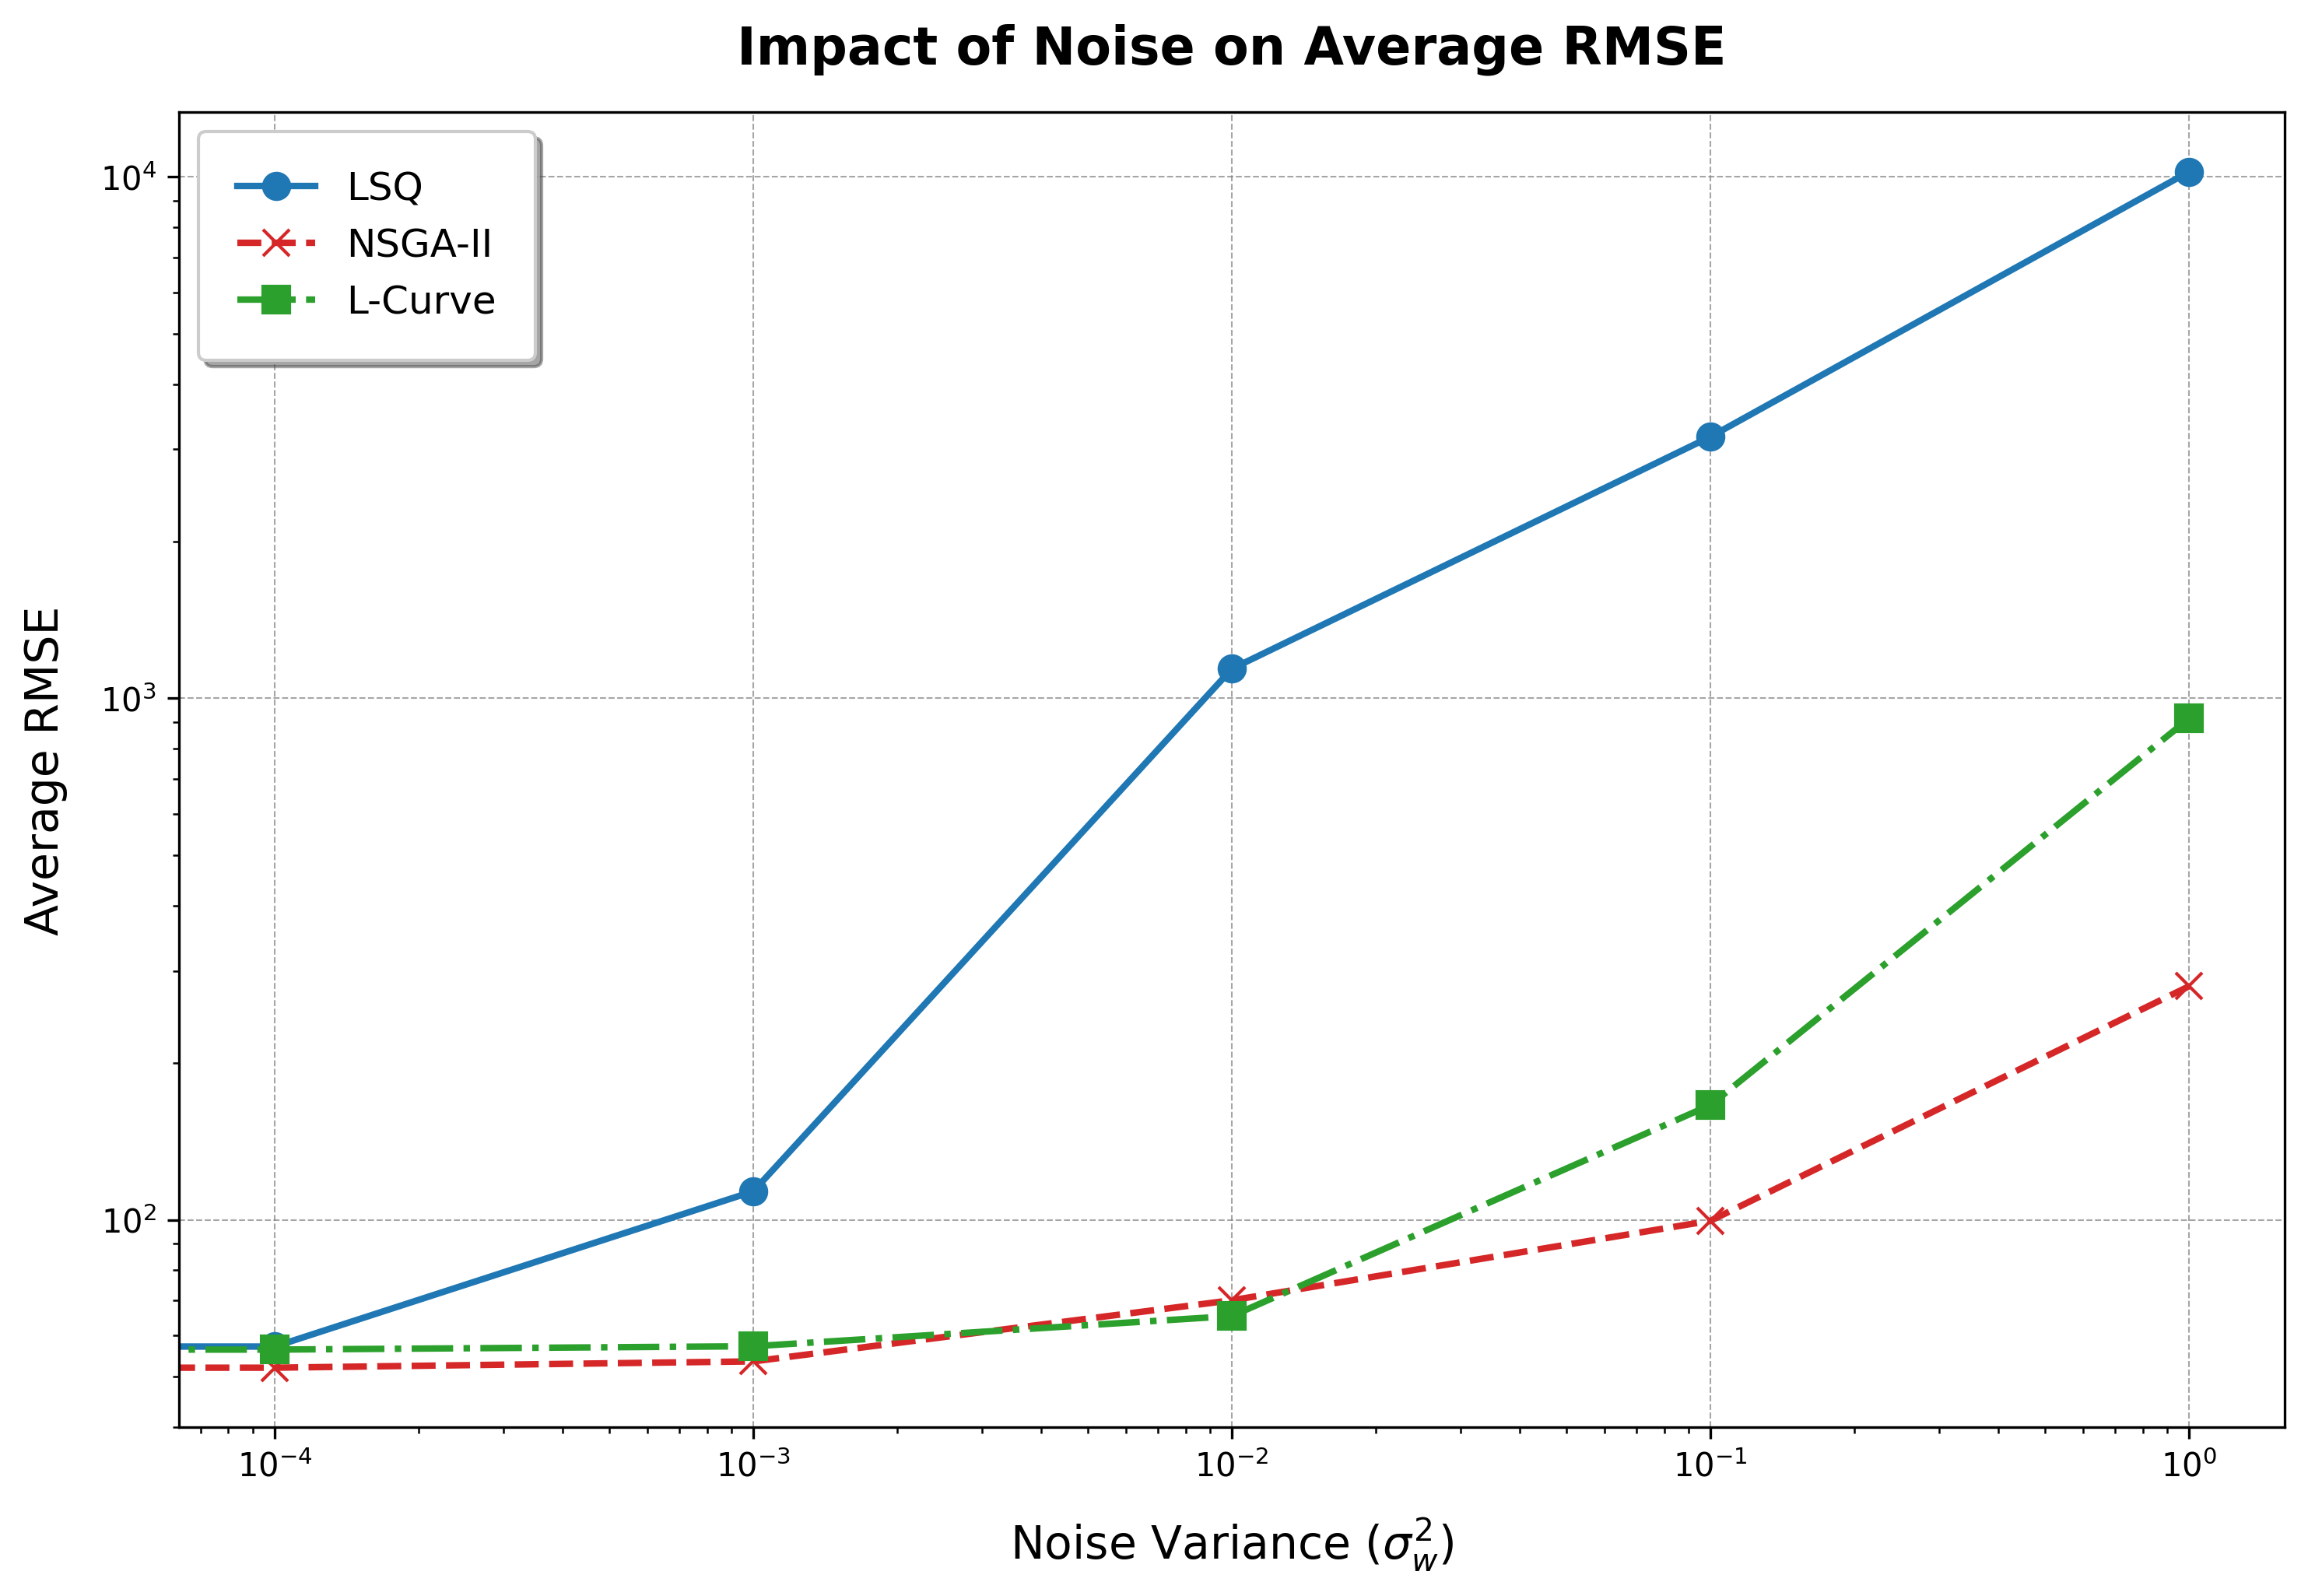
\includegraphics[width=0.8\textwidth]{Images/impact_noise_on_rmse_nsga2.png}
    \caption{Impacto del ruido en el RMSE promedio utilizando NSGA-II para diferentes valores de \( \sigma^2 \).}
    \label{fig:rmse_nsga2}
\end{figure}

\begin{figure}[H]
    \centering
    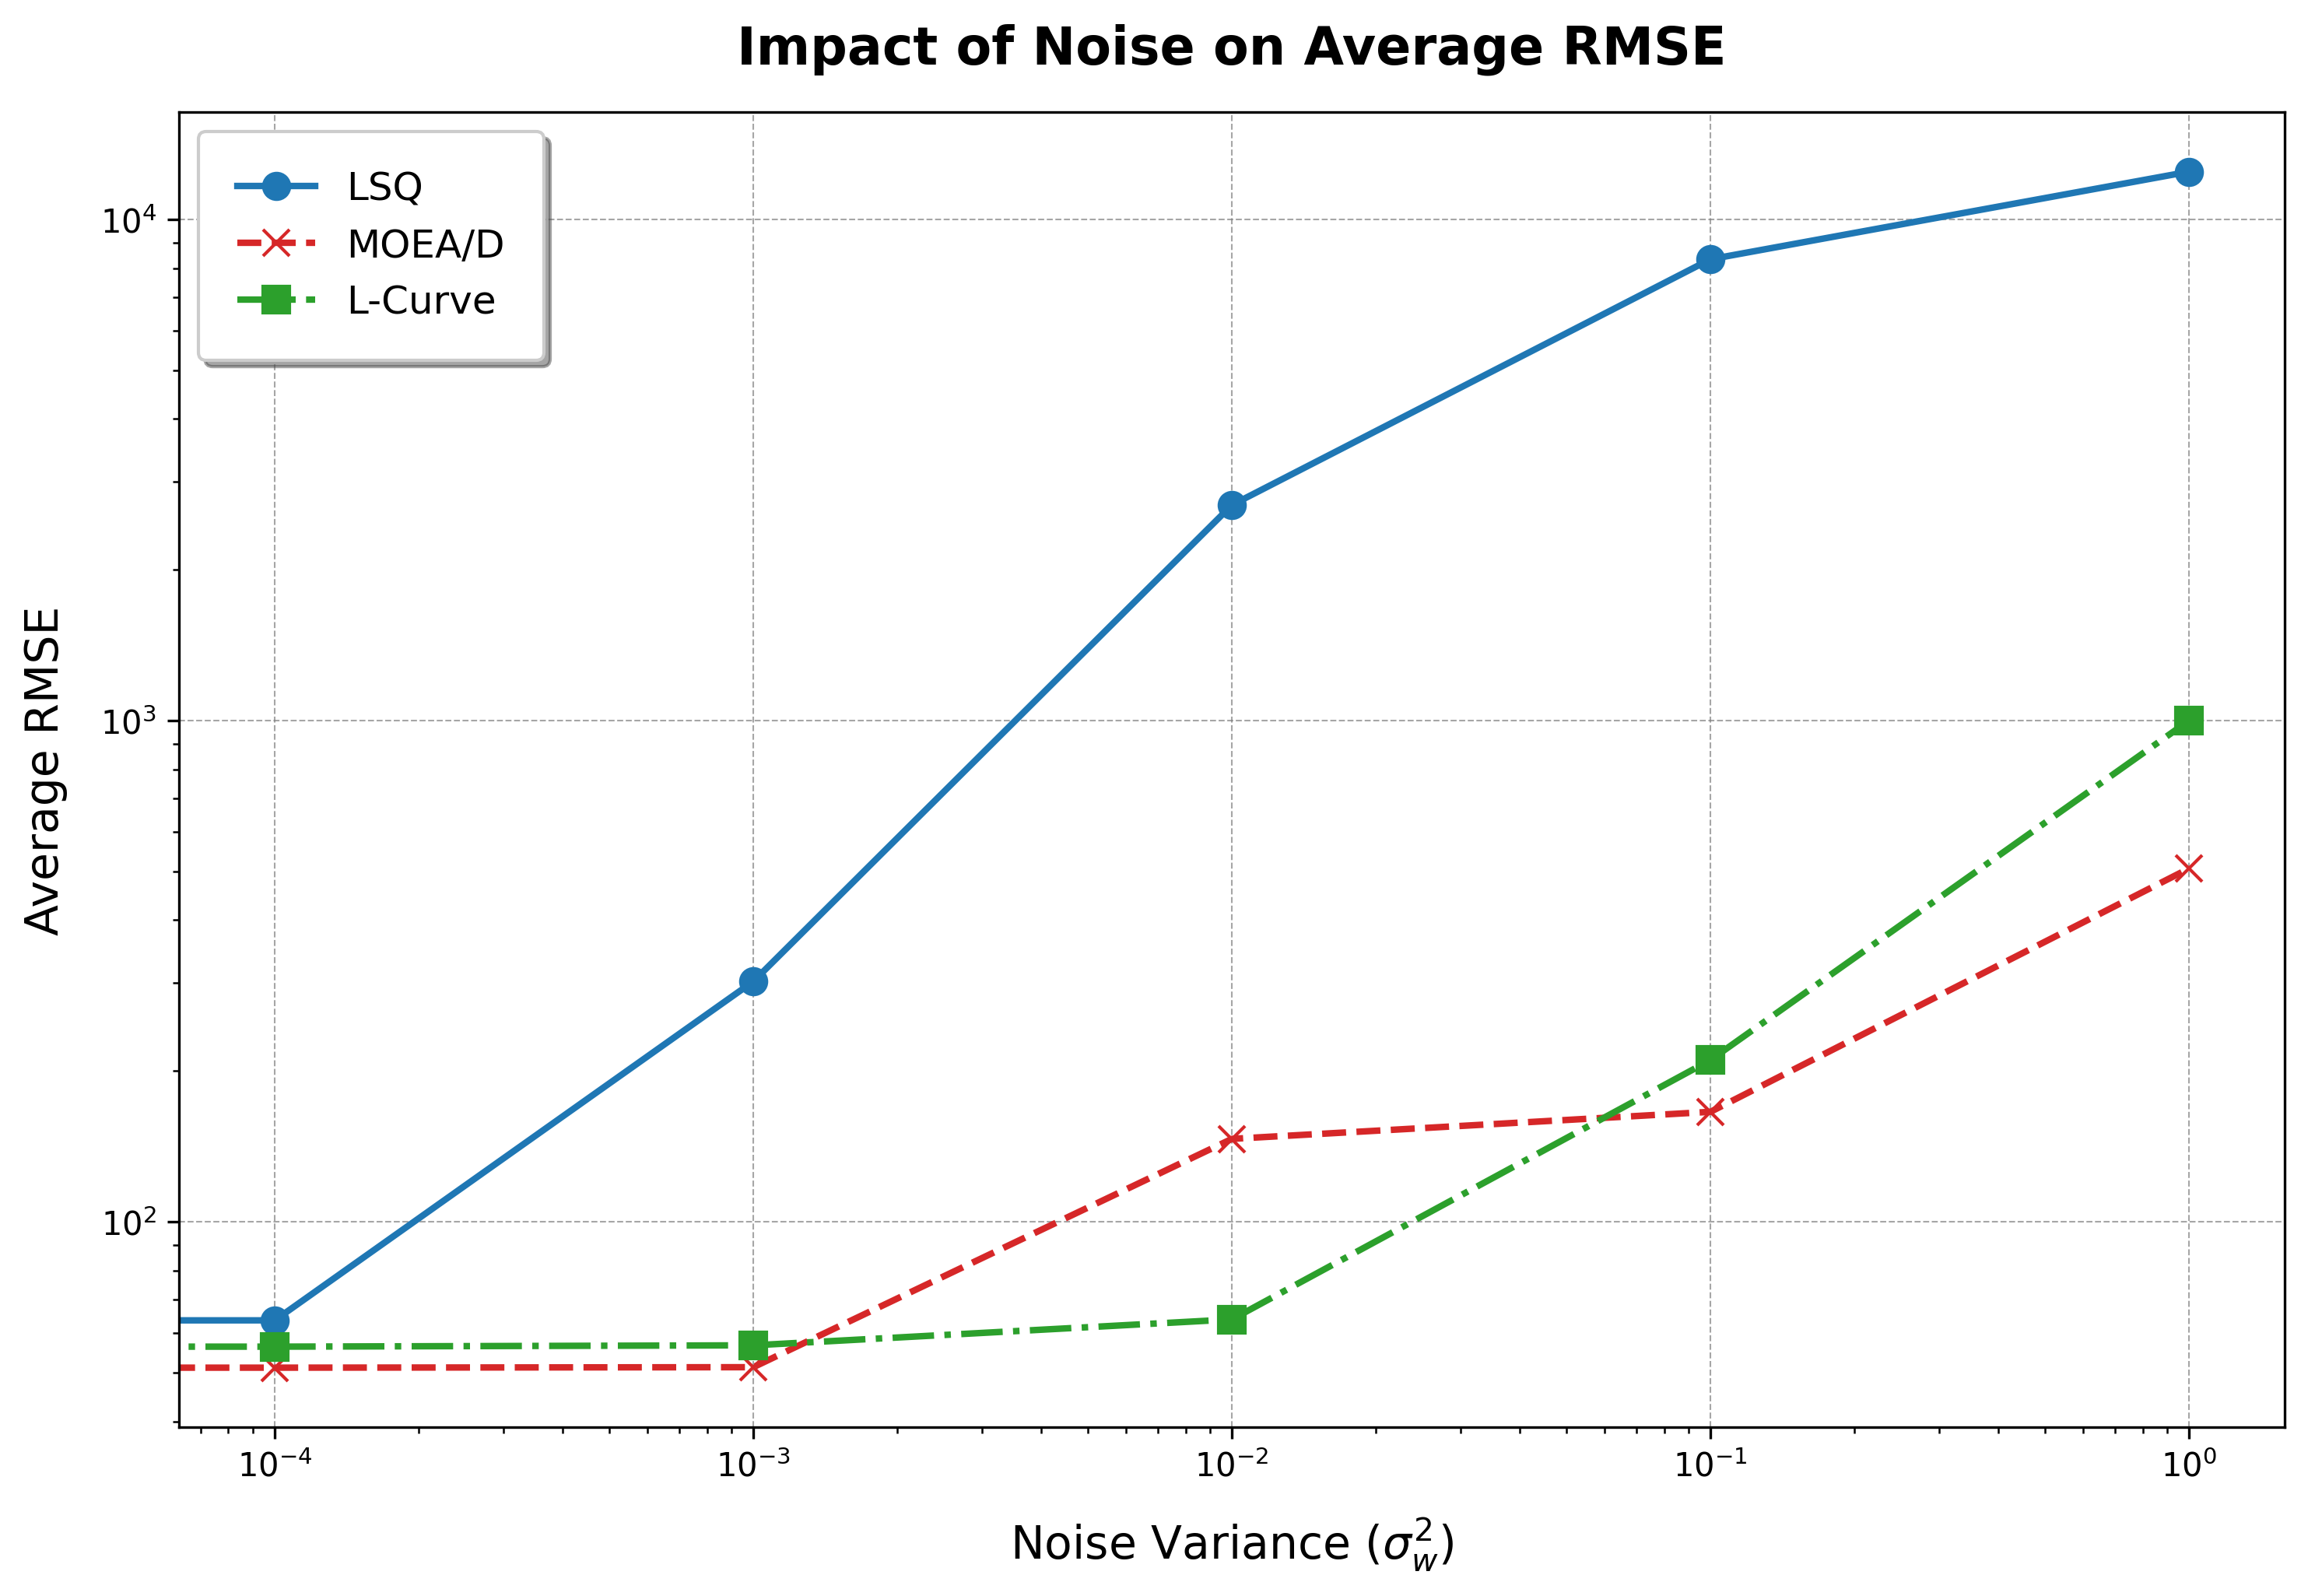
\includegraphics[width=0.8\textwidth]{Images/impact_noise_on_rmse_moead.png}
    \caption{Impacto del ruido en el RMSE promedio utilizando MOEA/D para diferentes valores de \( \sigma^2 \).}
    \label{fig:rmse_moead}
\end{figure}

Observaciones clave:
\begin{itemize}
    \item NSGA-II mantiene un RMSE más estable incluso en niveles altos de ruido, demostrando mejor adaptabilidad en condiciones adversas.
    \item MOEA/D es robusto a niveles bajos y moderados de ruido, pero muestra mayor sensibilidad para \( \sigma^2 > 10^{-1} \).
\end{itemize}


\section{Correlaciones entre Objetivos y Proyecciones en 2D} \label{sec:results:correlation}

Para interpretar mejor los compromisos entre los objetivos definidos (\(f_1\), \(f_2\), \(f_3\)), se analizaron las correlaciones entre ellos y se visualizaron las proyecciones en 2D de los frentes de Pareto generados por NSGA-II y MOEA/D.

\subsubsection{Correlaciones entre Objetivos}

La Figura \ref{fig:correlation_matrix} presenta la matriz de correlación entre las funciones objetivo \( f_1 \) (residual), \( f_2 \) (regularización) y \( f_3 \) (penalización de valores negativos), calculada utilizando las soluciones del frente de Pareto generado por MOEA/D y NSGA-II para \( \sigma^2 = 10^{-1} \).

\begin{figure}[H]
    \centering
    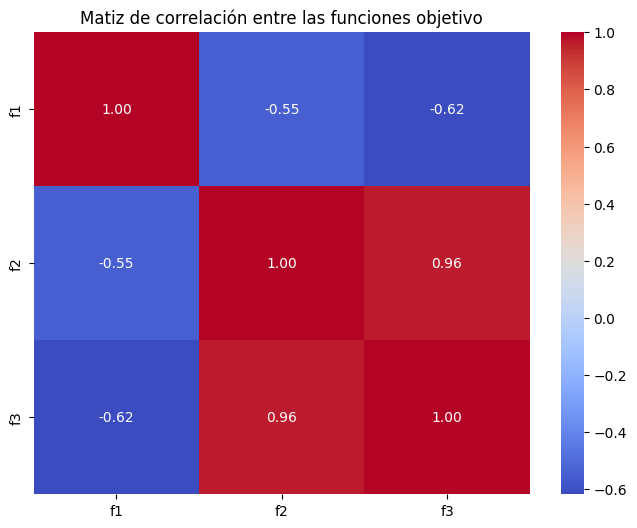
\includegraphics[width=0.7\textwidth]{Images/correlation_matrix.png}
    \caption{Matriz de correlación entre las funciones objetivo \( f_1 \), \( f_2 \), y \( f_3 \).}
    \label{fig:correlation_matrix}
\end{figure}

Los resultados destacan las siguientes tendencias clave:
\begin{itemize}
    \item Existe una correlación negativa entre \( f_1 \) y \( f_3 \) (\(-0.62\)) y entre \( f_1 \) y \( f_2 \) (\(-0.55\)), lo que refleja un compromiso entre minimizar el residual y garantizar soluciones físicamente consistentes.
    \item Se observa una alta correlación positiva entre \( f_2 \) y \( f_3 \) (\(0.96\)), lo que sugiere que aumentar la regularización también promueve soluciones con menor penalización por valores negativos.
    \item Estos patrones indican que los objetivos no son completamente independientes, y los algoritmos deben gestionar cuidadosamente estas correlaciones al explorar el espacio de soluciones.
\end{itemize}

Este análisis permite identificar relaciones entre objetivos, lo que facilita priorizar soluciones específicas según las necesidades de la aplicación.

\section{Proyecciones en 2D de los Objetivos}

\subsection{Proyecciones en 2D de los Objetivos (NSGA-II)}

Para analizar las relaciones entre los objetivos definidos, se realizaron proyecciones bidimensionales de las soluciones obtenidas con NSGA-II en el frente de Pareto. La Figura \ref{fig:objective_projections_nsga2} muestra las distribuciones marginales de cada objetivo (\(f_1\), \(f_2\) y \(f_3\)) en las diagonales principales, y los diagramas de dispersión para cada par de objetivos en las subgráficas restantes.

\begin{figure}[H]
    \centering
    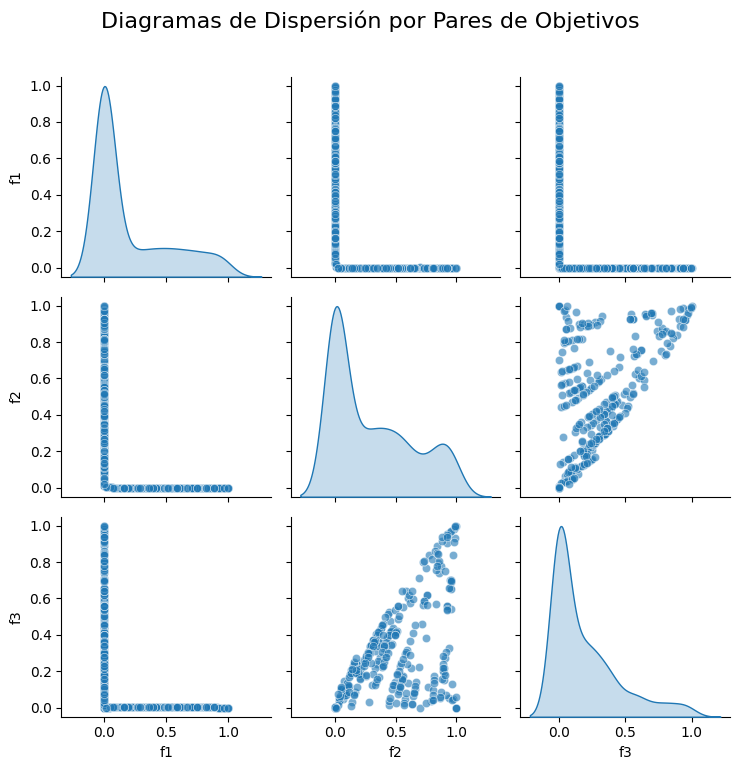
\includegraphics[width=0.9\textwidth]{Images/pareto_projection_nsga2.png}
    \caption{Proyecciones en 2D entre los objetivos \( f_1 \), \( f_2 \) y \( f_3 \) para NSGA-II. Cada subgráfica representa la relación entre dos objetivos, mientras que las distribuciones marginales se encuentran en la diagonal.}
    \label{fig:objective_projections_nsga2}
\end{figure}

\textbf{Observaciones clave:}
\begin{itemize}
    \item La relación entre \(f_2\) (regularización) y \(f_3\) (penalización de negatividad) es aproximadamente lineal, lo que confirma la correlación positiva observada en la matriz de correlación.
    \item \(f_1\) (residual) muestra una dispersión no lineal con respecto a \(f_2\) y \(f_3\), destacando compromisos complejos entre la fidelidad de los datos y la estabilidad de las soluciones.
    \item Las distribuciones marginales muestran una fuerte concentración de soluciones en valores bajos de \(f_1\) y \(f_3\), indicando que NSGA-II prioriza soluciones con bajos residuos y consistencia física.
\end{itemize}

\subsection{Proyecciones en 2D de los Objetivos (MOEA/D)}

Para MOEA/D, las proyecciones bidimensionales de los objetivos muestran relaciones distintivas en comparación con NSGA-II. La Figura \ref{fig:objective_projections_moead} presenta las distribuciones marginales de \(f_1\), \(f_2\) y \(f_3\) en la diagonal principal, junto con diagramas de dispersión para cada par de objetivos.

\begin{figure}[H]
    \centering
    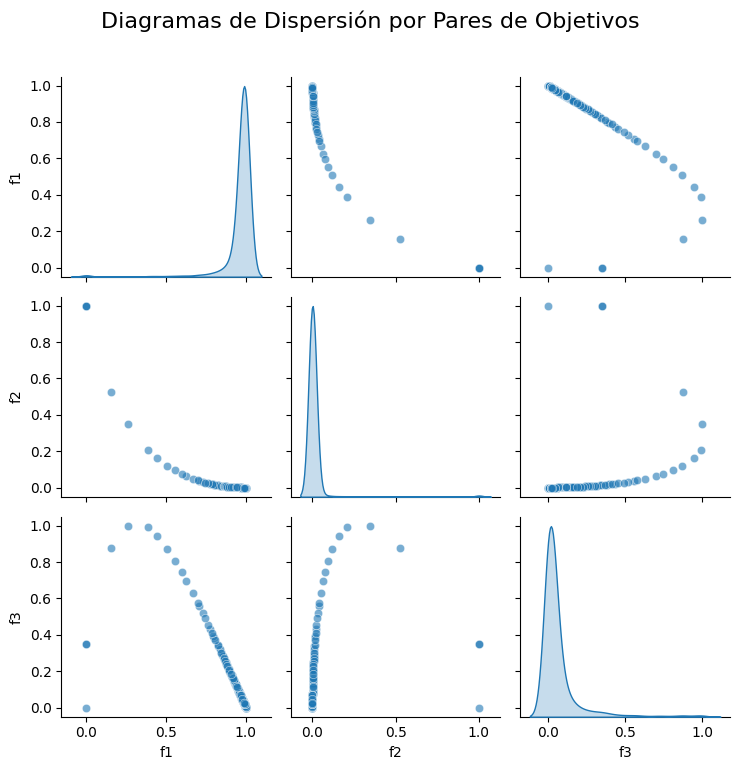
\includegraphics[width=0.9\textwidth]{Images/pareto_projection_moead.png}
    \caption{Proyecciones en 2D entre los objetivos \( f_1 \), \( f_2 \) y \( f_3 \) para MOEA/D. Las distribuciones marginales están en la diagonal principal, mientras que las relaciones entre pares de objetivos se muestran en las subgráficas.}
    \label{fig:objective_projections_moead}
\end{figure}

\textbf{Observaciones clave:}
\begin{itemize}
    \item La relación entre \(f_2\) (regularización) y \(f_3\) (penalización de negatividad) muestra una fuerte correlación no lineal, indicando una interacción más controlada entre estos objetivos.
    \item A diferencia de NSGA-II, \(f_1\) (residual) presenta una tendencia más estructurada en relación con \(f_2\), sugiriendo que MOEA/D logra una asignación más equilibrada en el frente de Pareto.
    \item Las distribuciones marginales son más uniformes en comparación con NSGA-II, lo que refleja el enfoque de descomposición de MOEA/D para generar soluciones equidistantes en el espacio objetivo.
\end{itemize}

\subsection{Comparación entre NSGA-II y MOEA/D}

El análisis de las proyecciones de los objetivos para NSGA-II (Figura \ref{fig:objective_projections_nsga2}) y MOEA/D (Figura \ref{fig:objective_projections_moead}) revela diferencias significativas en cómo estos algoritmos exploran el espacio de soluciones:
\begin{itemize}
    \item NSGA-II tiende a priorizar la diversidad en regiones dominadas por \(f_1\), mientras que MOEA/D genera frentes más uniformes con una mejor representación de \(f_2\) y \(f_3\).
    \item MOEA/D presenta una estructura más definida entre los objetivos, lo que puede ser ventajoso para problemas que requieren soluciones equitativas en el frente.
    \item En aplicaciones donde la positividad y la estabilidad son críticas, MOEA/D muestra un mejor desempeño debido a su habilidad para equilibrar \(f_3\) (penalización de negatividad).
\end{itemize}

